
%\documentclass[journal, draft]{IEEEtran} %%% draft mode WITHOUT graphics (puts every individual package in draft mode); hyperlinks DO NOT work here
%\documentclass[journal, draftcls]{IEEEtran} %%% draft mode WITH graphics
%\documentclass[journal, draftclsnofoot]{IEEEtran} %%% draft mode WITH graphics but without 'date + DRAFT' in footer
\documentclass[journal]{IEEEtran} %%% final

%%%%%%%%%%%%%%%%%%%%%%%%%
%%% {IEEEtran} is supposed to be compiled with 'pdflatex'
%%% if you want to use it with 'lualatex' for pgfplots from python
%%% to not run out of memory
%%% 'dvips' has to be commented!!
%%% see this https://texfaq.org/FAQ-nonpdfsp
%	\ifCLASSINFOpdf
%	\else
%	   \usepackage[dvips]{graphicx}
%	\fi
%%%
%%%%%%%%%%%%%%%%%%%%%%%%%

\usepackage[hyphens]{url}

\hyphenation{op-tical net-works semi-conduc-tor}

\usepackage{graphicx}


%%% my own additions %%%
%\usepackage[smaller, printonlyused]{acronym}%%% for nice acroym table
\usepackage[nolist]{acronym}%%% for acroyms WITHOUT the table
\usepackage{subcaption}%%% for subfigure (automatically loads {caption} as well
\usepackage{overpic}%%% to be able to write in latex font over a picture
\usepackage{siunitx}%%% for easy si units
\usepackage{amsmath}%%% for equation and align environment, nicely aligned multiline equations 
\usepackage{amssymb}%%% for math symbols
%%% messes with ieee template \IEEEsetlabelwidth %\usepackage{enumitem}%%% for enumerate environment but with a, b, c (https://tex.stackexchange.com/questions/129951/enumerate-tag-using-the-alphabet-instead-of-numbers)
\usepackage{cite}%%% for citation range [3-6] instead of [3], [4], [5], [6]
%%% the lidar market overview
\usepackage{multirow}%%% for tabular with multi row
\usepackage{float}%%% to be able to enforce location of table with the [H] option
\usepackage{makecell}%%% needed for cornis cnn tikz figure

%%%%%%%%%%%%%%%%%%%%%%%%%%%%%%%%%%%
%%% used for lidar design space %%%
%%%%%%%%%%%%%%%%%%%%%%%%%%%%%%%%%%%
\usepackage{environ}
\makeatletter
\newsavebox{\measure@tikzpicture}
\NewEnviron{scaletikzpicturetowidth}[1]{%
  \def\tikz@width{#1}%
  \def\tikzscale{1}\begin{lrbox}{\measure@tikzpicture}%
  \BODY
  \end{lrbox}%
  \pgfmathparse{#1/\wd\measure@tikzpicture}%
  \edef\tikzscale{\pgfmathresult}%
  \BODY
}
\makeatother
%%%%%%%%%%%%%%%%%%%%%%%%%%%%%%%%%%%%%%%%%
\usepackage{pdfpages}%%% to include pdf pages in lidar market overview
\usepackage{pgfplots}%%% including .pgf plots from matplotlib (python); I guess it also loads {pgf} and {tikz}
\usepackage{tikz-3dplot}%%% tikz 3d plotting, formally known as \usepackage{3dplot}, can still be found on web
\pgfplotsset{compat=1.16}%%% suggested by pgfplots package 
\usetikzlibrary{calc, quotes, angles, arrows.meta}%%% this is needed for nice angles; arrows.meta from stress strain f arrows in mems part
%\usetikzlibrary{shapes.geometric, arrows}%%% this is needed for flow charts
%\usetikzlibrary{patterns}%%% this is needed for gaussian


%%% for nicer hyperlinks! %%%
%% Hyperlinks im Dokument; muss als eines der letzten Pakete geladen werden
\usepackage[pdfstartview=FitH,      % Oeffnen mit fit width
            breaklinks=true,        % Umbrueche in Links, nur bei pdflatex default
            bookmarksopen=true,     % aufgeklappte Bookmarks
            bookmarksnumbered=true, % Kapitelnummerierung in bookmarks
            hidelinks]{hyperref}	%%% HIDE LINKS HABE ICH EINGEFUEGT!
%\hypersetup{			%%% hier definiere ich
%    colorlinks,			%%% die farbe fuer clickable
%    linkcolor={red!80!black},	%%% words instead of the 
%    citecolor={green!50!black},	%%% ugly boxes
%    urlcolor={blue!80!black}
%}

%%% glossaries has to be loaded after hyperref
%%% if you wanna use clickable entries, see manual in referencer
\usepackage[nopostdot]{glossaries}



%% Ibeo Colors
\definecolor{R}{rgb}{0.819608, 0.054902, 0.133333}%Ibeo Red
\definecolor{W}{rgb}{1, 1, 1}%Ibeo White
\definecolor{G}{rgb}{0.698039, 0.682353, 0.686275}%Ibeo Gray
\definecolor{B}{rgb}{0.2, 0.2, 0.2}%Ibeo Black

%% fast typing
\newcommand{\ie}{i.e.\ }
\newcommand{\Ie}{I.e.\ }
\newcommand{\eg}{e.g.\ }
\newcommand{\Eg}{E.g.\ } 
\newcommand{\cf}{cf.\ } 

%% math commands
\DeclareMathOperator\erf{erf}
\DeclareMathOperator\erfc{erfc}

%%%%%%%%%%%%%%%%%%%%%%%%
%%% used for heating %%%
%%%%%%%%%%%%%%%%%%%%%%%%
\newcommand{\dC}{\unit{\degreeCelsius}}




\begin{document}

%%% input table of contents
%\tableofcontents
%%% input acronyms table
%\section*{Acronyms} %%% include if caption wanted
%%% if \ac{[...]} is used, 
%%% ALL CAPITAL SINCE ACROS ARE ALSO CAPITAL
%%% MATCH BIG LETTERS

%%% from \cite{Michael15}
%%% but my acronym table looks good
%\renewcommand{\IEEEiedlistdecl}{\IEEEsetlabelwidth{SONET}}

\begin{acronym}[TCSPC] %%% HERE [ *** ] insert longest acronym (for spacing)
\acro{1D}{one-dimensional}
\acro{2D}{two-dimensional}
\acro{3D}{three-dimensional}
\acro{3PPC}{3-Peak Point Cloud}
\acro{AC}{Alternating Current}
\acro{ADAS}{Advanced Driver-Assistance Systems}
\acro{ADC}{Analog-to-Digital Converter}
\acro{ALU}{Arithmetic Logic Unit}
\acro{AMCW}{Amplitude Modulated Continuous Wave}
\acro{APD}{Avalanche Photo Diode}
\acro{ASIC}{Application-Specific Integrated Circuit}
\acro{BOM}{Bill of Material}
\acro{BS}{Beam Splitter}
\acro{CFD}{Constant Fraction Discriminator}
\acro{CNN}{Convolutional Neural Network}
\acro{DC}{Direct Current}
\acro{DCR}{Dark Count Rate}
\acro{DSP}{Digital Signal Processing}
\acro{ECU}{Electronic Control Unit}
\acro{EEL}{Edge-Emitting Laser}
\acro{EMG}{Exponentially Modified Gaussian}
\acro{FC}{Fog Classifier}
\acro{FFT}{Fast Fourier Transform}
\acro{FMCW}{Frequency Modulated Continuous Wave}
\acro{FOV}{Field Of View}
\acro{FPA}{Focal Plane Array}
\acro{FPGA}{Field Programmable Gate Array}
\acro{FPI}{Fog Peak Identifier}
\acro{FWHM}{Full Width at Half Maximum}
\acro{FR}{Fog Recognizer}
\acro{GSps}{Giga Samples per second}
\acro{HIL}{Hardware in the Loop}
\acro{InGaAs}{Indium Gallium Arsenide}
\acro{KPI}{Key Performance Indicator}
\acro{LC}{Liquid Crystal}
\acro{LiDAR}{Light Detection and Ranging}
\acro{LO}{Local Oscillator}
\acro{LUT}{Lookup Table}
\acro{MEMS}{Micro-Electro-Mechanical System}
\acro{NIR}{Near Infrared}
\acro{OPA}{Optical Phased Array}
\acro{PBS}{Polarizing Beam Splitter}
\acro{PDF}{Probability Density Function}
\acro{PG}{Polarization Grating}
\acro{PIC}{Photonic Integrated Circuits}
\acro{PIN}{Positive Intrinsic Negative}
\acro{PO}{Power Oscillator}
\acro{POC}{Proof Of Concept}
\acro{RaDAR}{Radio Detection And Ranging}
\acro{ReLU}{Rectified Linear Unit}
\acro{ScaLa}{Scanning Laser}
\acro{SH}{Smoothed Histogram}
\acro{SLM}{Spatial Light Modulator}
\acro{SNR}{Signal-to-Noise Ratio}
\acro{SPAD}{Single-Photon Avalanche Diode}
\acro{SPPC}{Single Peak Point Cloud}
\acro{SWIR}{Short-Wave Infrared}
\acro{TIA}{Transimpedance Amplifier}
\acro{TCSPC}{Time-Correlated Single Photon Counting}
\acro{TDC}{Time-to-Digital Converter}
\acro{TOF}{Time-Of-Flight}
\acro{TRL}{Technology Readiness Level}
\acro{VCSEL}{Vertical-Cavity Surface Emitting Laser}
\end{acronym} 

%\renewcommand{\IEEEiedlistdecl}{\relax}% reset back

 has to always be here 

%%% ALL CAPITAL SINCE ACROS ARE ALSO CAPITAL
%%% MATCH BIG LETTERS

%%% from \cite{Michael15}
%%% but my acronym table looks good
%\renewcommand{\IEEEiedlistdecl}{\IEEEsetlabelwidth{SONET}}

\begin{acronym}[TCSPC] %%% HERE [ *** ] insert longest acronym (for spacing)
\acro{1D}{one-dimensional}
\acro{2D}{two-dimensional}
\acro{3D}{three-dimensional}
\acro{3PPC}{3-Peak Point Cloud}
\acro{AC}{Alternating Current}
\acro{ADAS}{Advanced Driver-Assistance Systems}
\acro{ADC}{Analog-to-Digital Converter}
\acro{ALU}{Arithmetic Logic Unit}
\acro{AMCW}{Amplitude Modulated Continuous Wave}
\acro{APD}{Avalanche Photo Diode}
\acro{ASIC}{Application-Specific Integrated Circuit}
\acro{BOM}{Bill of Material}
\acro{BS}{Beam Splitter}
\acro{CFD}{Constant Fraction Discriminator}
\acro{CNN}{Convolutional Neural Network}
\acro{DC}{Direct Current}
\acro{DCR}{Dark Count Rate}
\acro{DSP}{Digital Signal Processing}
\acro{ECU}{Electronic Control Unit}
\acro{EEL}{Edge-Emitting Laser}
\acro{EMG}{Exponentially Modified Gaussian}
\acro{FC}{Fog Classifier}
\acro{FFT}{Fast Fourier Transform}
\acro{FMCW}{Frequency Modulated Continuous Wave}
\acro{FOV}{Field Of View}
\acro{FPA}{Focal Plane Array}
\acro{FPGA}{Field Programmable Gate Array}
\acro{FPI}{Fog Peak Identifier}
\acro{FWHM}{Full Width at Half Maximum}
\acro{FR}{Fog Recognizer}
\acro{GSps}{Giga Samples per second}
\acro{HIL}{Hardware in the Loop}
\acro{InGaAs}{Indium Gallium Arsenide}
\acro{KPI}{Key Performance Indicator}
\acro{LC}{Liquid Crystal}
\acro{LiDAR}{Light Detection and Ranging}
\acro{LO}{Local Oscillator}
\acro{LUT}{Lookup Table}
\acro{MEMS}{Micro-Electro-Mechanical System}
\acro{NIR}{Near Infrared}
\acro{OPA}{Optical Phased Array}
\acro{PBS}{Polarizing Beam Splitter}
\acro{PDF}{Probability Density Function}
\acro{PG}{Polarization Grating}
\acro{PIC}{Photonic Integrated Circuits}
\acro{PIN}{Positive Intrinsic Negative}
\acro{PO}{Power Oscillator}
\acro{POC}{Proof Of Concept}
\acro{RaDAR}{Radio Detection And Ranging}
\acro{ReLU}{Rectified Linear Unit}
\acro{ScaLa}{Scanning Laser}
\acro{SH}{Smoothed Histogram}
\acro{SLM}{Spatial Light Modulator}
\acro{SNR}{Signal-to-Noise Ratio}
\acro{SPAD}{Single-Photon Avalanche Diode}
\acro{SPPC}{Single Peak Point Cloud}
\acro{SWIR}{Short-Wave Infrared}
\acro{TIA}{Transimpedance Amplifier}
\acro{TCSPC}{Time-Correlated Single Photon Counting}
\acro{TDC}{Time-to-Digital Converter}
\acro{TOF}{Time-Of-Flight}
\acro{TRL}{Technology Readiness Level}
\acro{VCSEL}{Vertical-Cavity Surface Emitting Laser}
\end{acronym} 

%\renewcommand{\IEEEiedlistdecl}{\relax}% reset back

 %%% \usepackage[!!] defines if table is included here or not


\title{Front Cover Thermodynamics}


\author{Tobias Rybka, Hanno Holzh{\"u}ter, Georg Schneider and Holger Blume%

%\thanks{Thanks Ibeo and IMS Uni Hannover ??}%

\thanks{T. Rybka (e-mail: tobias.rybka@ibeo-as.com-hannover.de) and G.
Schneider are with Ibeo AS, Merkurring 60-62, 22143 Hamburg, Germany}%

\thanks{H. Holzh{\"u}ter is with Ibeo AS, Merkurring 60-62, 22143 Hamburg,
Germany and the Institute of Microelectronic Systems (IMS) at Leibniz
University Hannover, Appelstraße 4, 30167 Hanover, Germany (e-mail:
hanno.holzhueter@ims.uni-hannover.de)}%

%\thanks{C. Hofs{\"a}{\ss} is with Ibeo AS, Merkurring 60-62, 22143 Hamburg,
%Germany}%

\thanks{H. Blume is the Head of Architectures and Systems Group at the
Institute of Microelectronic Systems (IMS) at Leibniz University Hannover,
Appelstraße 4, 30167 Hanover, Germany}%
}

\markboth{Journal of \LaTeX\ Class Files, Vol. 14, No. 8, August 2015}
{Shell \MakeLowercase{\textit{et al.}}: Bare Demo of IEEEtran.cls for IEEE Journals}
\maketitle

\begin{abstract}
Deicing of an automotive sensor for autonomous driving is necessary to provide
a clear sight. The heat generated by a sensor itself typically is not
sufficient for defrosting ice accumulated on the outer surface at low
temperatures and high wind speeds. This results in a need for integrating an
active heating element in the system. Finding the right heating layout can be a
complex problem that is shaped by the requirement to maintain the optical
quality during heating and to achieve a high heating performance in parallel.
Every design must be verified to meet this goal and the verification is usually
achieved by a sophisticated simulation or experiment. The aim of this study is
to ease the verification process by providing a description of the heat flow in
a plane front cover design with different heating layouts and finding a
(semi-)analytical expression for the surface temperature as a function of the
heating power, ambient temperature and wind speed. Only steady conditions and
temperatures are considered. The model accuracy is demonstrated for the Ibeo
NEXT LiDAR sensor. In addition, a numerical FEM analysis is performed to verify
the results in a 3D model.
% \\
% A single paragraph of about 200 words maximum. For research articles,
% abstracts should give a pertinent overview of the work. We strongly encourage
% authors to use the following style of structured abstracts, but without
% headings: (1) Background: Place the question addressed in a broad context and
% highlight the purpose of the study; (2) Methods: Describe briefly the main
% methods or treatments applied; (3) Results: Summarize the article's main
% findings; and (4) Conclusion: Indicate the main conclusions or
% interpretations. The abstract should be an objective representation of the
% article, it must not contain results which are not presented and
% substantiated in the main text and should not exaggerate the main
% conclusions.
\end{abstract}

\begin{IEEEkeywords}
sensor front cover heating; deicing; all weather sensing; automotive LiDAR
\end{IEEEkeywords}

\IEEEpeerreviewmaketitle



\newcommand{\pathPics}{heating_files/Pictures/}

%!TEX root = 0_document_de.tex
\section{Scope}

Active opitcal sensors play an important role in perception systems of
autonomous driving cars.
Their datas availability is crucial for safe driving operations.
This is true under all weather conditions conditions which causes a need for
heating and cleaning mechanism for such sensors.
In this work we present the theoretical bases to design a heating system for an
active optical sensor.
Furhtermore, an example configuration for an automotive \ac{LiDAR} sensor is
provided for the deicing use-case.

\begin{figure} [H]
  \centering
  \begin{tikzpicture}
    \node[anchor=south west,inner sep=0] (image) at (0,0,0) {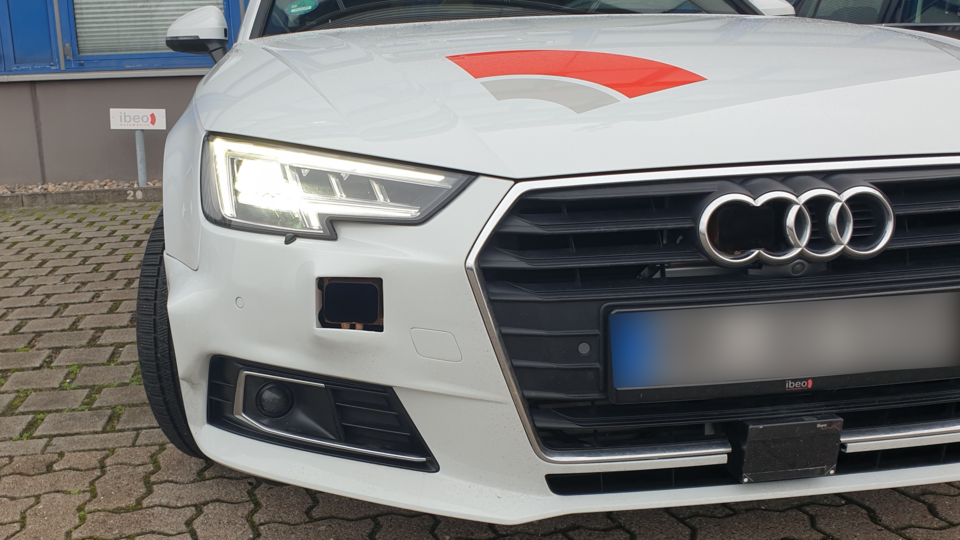
\includegraphics[width=0.45\textwidth]{\pathPics/2021-12-07_car_b0-rot_number-plate_blurred_reduced.png}};
    \begin{scope}[x={(image.south east)},y={(image.north west)}]
      \node[anchor=west, R] (s) at (0.35, 0.775) {ibeoNEXT};
      \draw[very thin, ->, > = latex, R] (s) -- (.41, .5);
      \draw (.365, .44) [thick, R] circle (2mm);
      \draw[very thin, ->, > = latex, R] (s) -- (.72, .62);
      \draw (.78, .575) [thick, R] circle (2mm);
    \end{scope}
  \end{tikzpicture}
  \caption{Sensors in car.}
  \label{fig:examples}
\end{figure}


Deicing of a LiDAR sensor is necessary to provide a clear sight.
The heat generated by a sensor itself is typically not sufficient for
defrosting ice accumulated on the outer surface (see appendix A.1).
That's true in particular at low temperatures and high wind speeds resulting in
a need for integrating an active heating element in the system.
Finding the right heating layout can be a complex problem that is shaped by the
requirement to maintain the optical quality during heating and to achieve a
high heating performance in parallel.
Which heating performance is required depends on use cases.
For deicing the system must be designed in such a way that the available
heating power is sufficient to heat up the surface temperature above \(0\dC\)
for a specified range of ambient temperatures and wind speeds.
Every design must be verified to meet this goal and the verification is usually
achieved by a sophisticated simulation or experiment.
The aim of this document is to ease the verification process by providing a
description of the heat flow in a plane front cover with different heating
layouts and finding a (semi-)analytical expression for the surface temperature.
Only steady conditions and temperatures are considered.
The model accuracy is demonstrated for the NEXT LiDAR sensor.
In addition, a Matlab script based on finite element analysis is provided to
solve the heat transfer problem for a 3-D model of the NEXT LiDAR front cover
(see appendix A.3). 

In general, the surface temperature depends on the following influences:

\underline{Environmental influences}
\begin{itemize}
\item Ambient temperature \(T_{o}\)
\item Relative wind speed \(v\)
\item Precipitation on the surface
\end{itemize}

\underline{Design and control parameters}
\begin{itemize}
\item Heating power \(P\) or temperature of the heating wire/plate \(T_{hs}\)
\item Front cover design (thickness, distance between wires, ...)
\item Material (composition) of the front cover
\item Internal heat transfer from the LiDAR sensor electronics to the surface
\item Mounting position (on the car)
\end{itemize}

\begin{figure} [H]
	\centering
	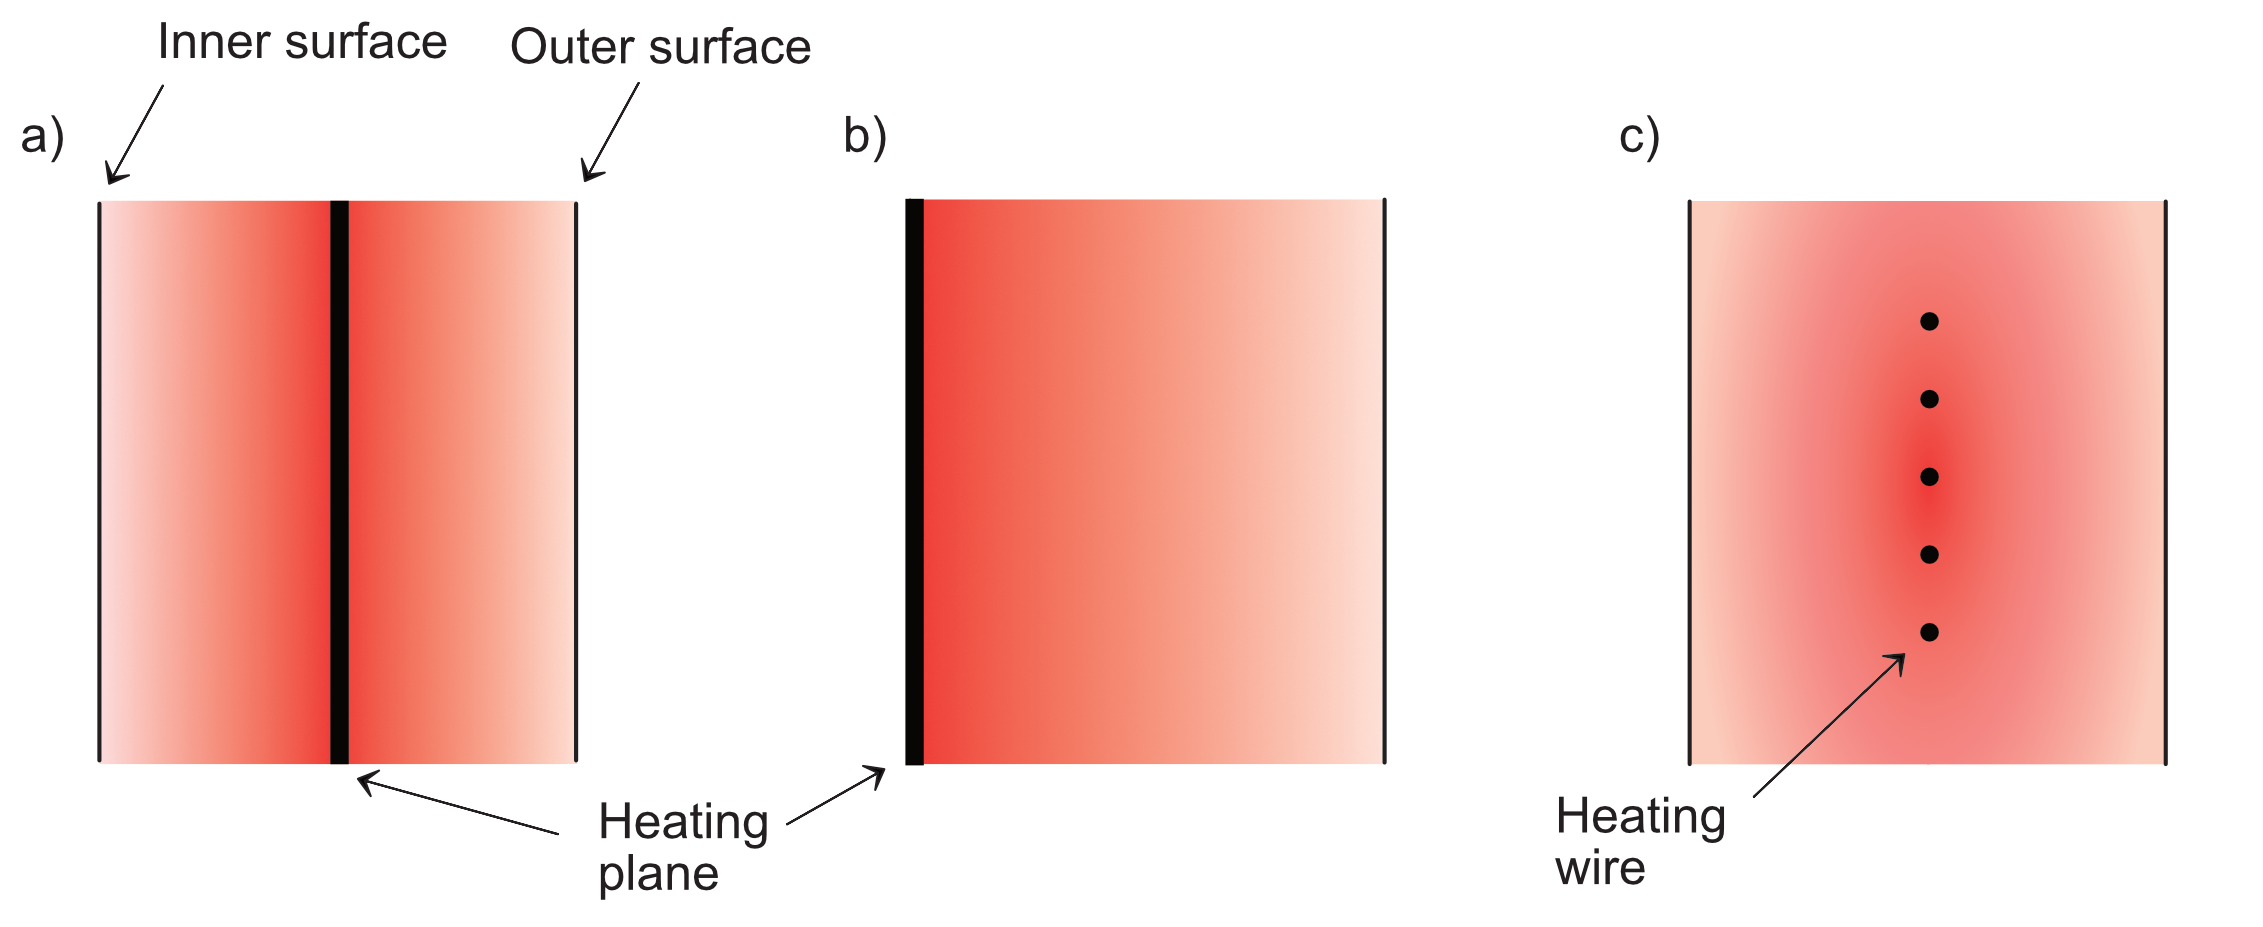
\includegraphics[scale=0.375]{\pathPics/FrontCoverTypes.png}

	\caption[Heating Architectures]{Side view on three front covers with different heating architectures where a) a heating plate is buried in the mid plane b) a heating plate is attached to the inner surface and c) a row of equally spaced parallel heating wires are buried in the mid plane.}
	\label{fig:examples}
\end{figure}


\section{Generic Thermodynamic Model}
In this section, a generic analytical expression for the surface temperature of a (LiDAR) sensor is derived as a function of relative wind speed, ambient temperature and the heating power applied to the heating element. The expression can be applied to planar front covers in thermodynamic equilibrium. 

Many thermodynamic problems encountered in practice are two- or three-dimensional and involve rather complicated geometries for which no simple solutions exist. The front cover of the NEXT sensor shown in Fig. \ref{fig:1TB1Model} is such an example. One-dimensional geometries have exact solutions. Figures \ref{fig:examples}a and \ref{fig:examples}b show the side view of two heating geometries of which simple analytical solutions can be derived. The geometry in Fig. \ref{fig:examples}c is a two-dimensional problem and requires a more elaborate calculation. Nonetheless, the solution is identical to the solution of the geometry in Fig. 1a when introducing a shape factor. This shape factor must be adjusted accordingly for more complex heating architectures such as the NEXT sensors front cover and can be found only numerically or experimentally. 

In the following, first the basic underlying thermodynamic expressions are introduced. Secondly, the surface temperature of the heating plate architecture shown in Fig. \ref{fig:examples}a is derived. Based on this solution, a general equation for more complex, planar geometries is derived by introducing the shape factor.

\subsection{Thermodynamic Model}\label{chapter:basics}
Figure \ref{fig:simpleplate} depicts a sketch of a wall with a temperature difference between the inner and outer side. The heat transferred per unit time, \(\dot Q\), through a solid wall of thickness \(d\) and area \(A\) depends on the temperature difference \(T_i - T_o\) between the inner side and the outer side of the wall:
\begin{equation}
\frac{\dot Q}{A} =  \frac{1}{R_{tot}}\cdot (T_i - T_o)
\end{equation}
with \(R_{tot}\) being the total thermal resistance of the wall. The higher the temperature difference and the lower the thermal resistance, the higher is the heat lost through the area per unit time. 

The heat is transferred by conduction through the wall and by convection of air and radiation from the inside to the wall and also from the wall to the outside. Heat transferred by radiation only needs to be considered if the temperatures in the system are very high and only natural convection occurs (no wind). The purpose of this heat transfer analysis is mainly to determine whether a chosen heating design is sufficient to deice the surface or not. For this we need to know the maximum rate of heat loss from the surface, which is determined by considering the heat loss from the surface under worst conditions for an extended period of time, that is, during steady operation under worst conditions. If the heating layout is good enough to deice the outer surface under most demanding conditions, i.e. at high winds and low temperatures, it is good enough for all conditions. At high wind speeds, the radiative heat transfer can be neglected. But even for low wind conditions, the radiative heat transfer rate is lower than the heat transferred by natural convection. Additionally, a layer of ice adds a layer of thermal resistance and lowers the necessary heat transfer rate to melt the ice. In this model, by omitting an additional layer of ice, the solution is more conservative. Nonetheless, the additional layer can be easily added to the model.

\begin{figure} [H]
	\centering
	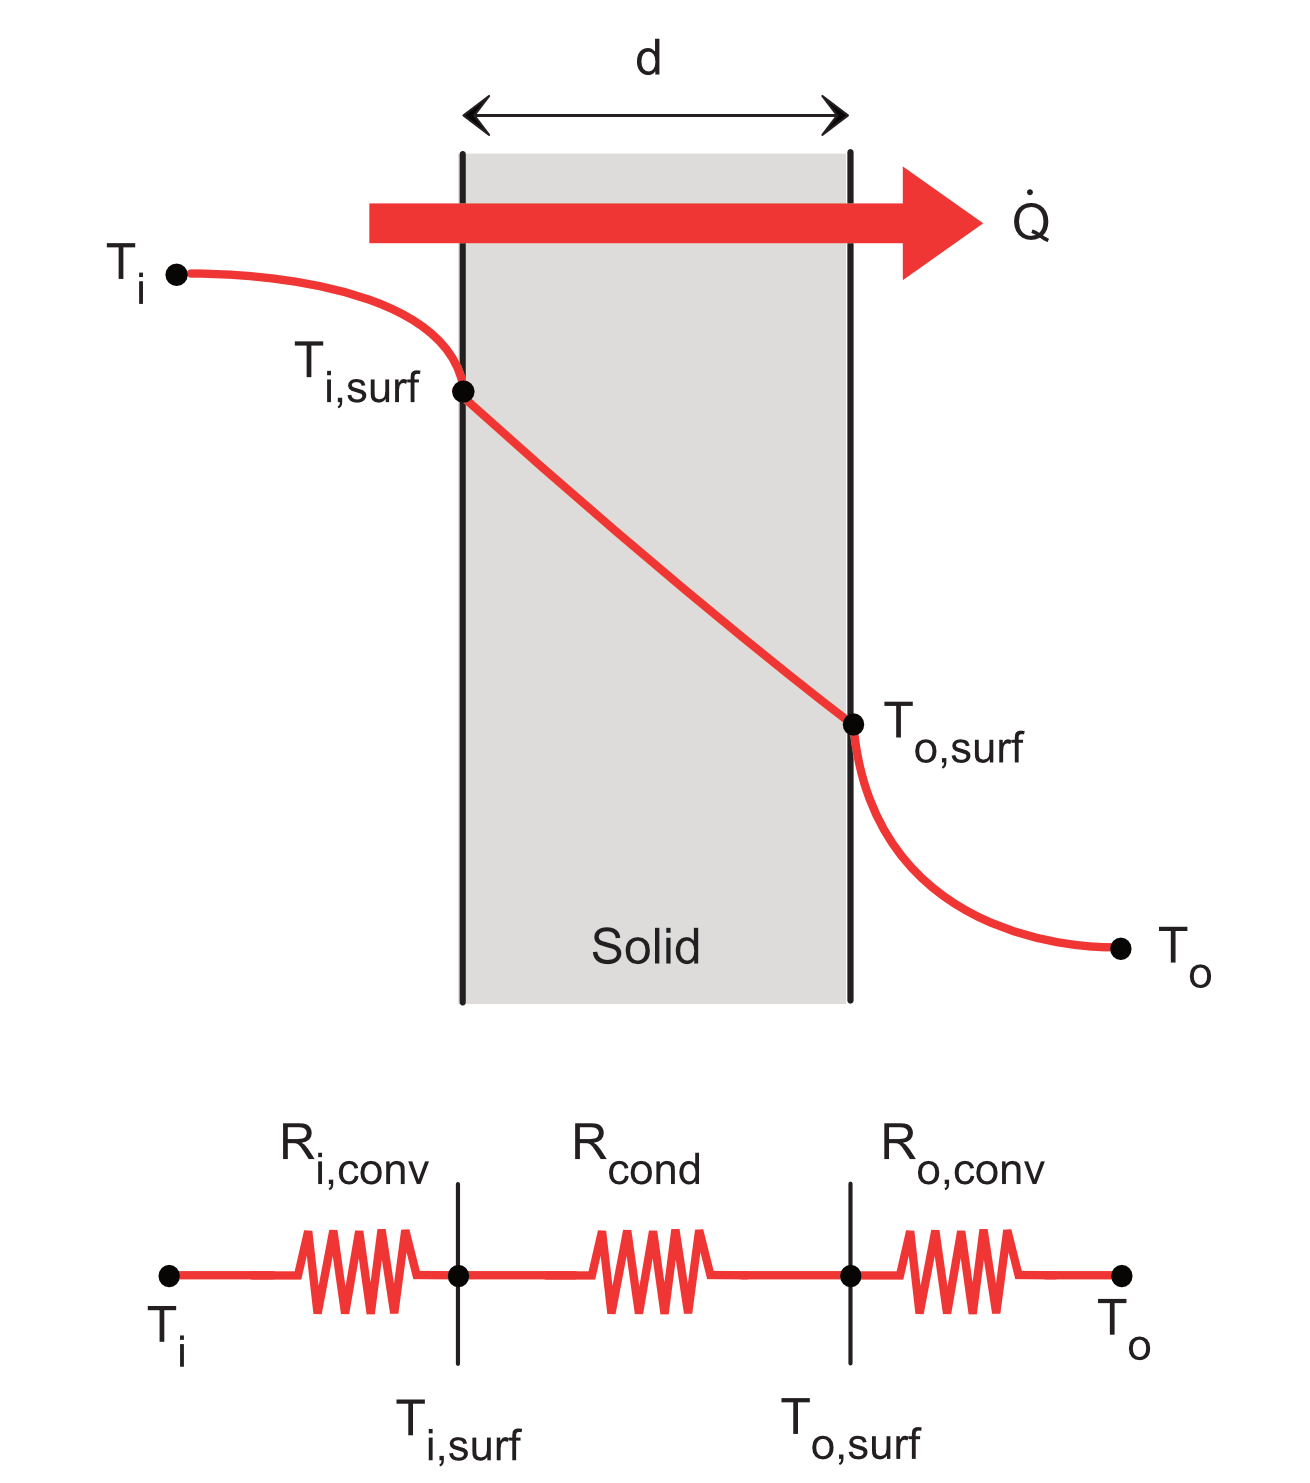
\includegraphics[scale=0.375]{\pathPics/SimplePlate.png}
	\caption[SimplePlate]{The upper parts shows the side view sketch of a solid with a qualitative temperature profile (red line) and heat flow (red arrow). The lower part shows an analogous electrical circuit.}
	\label{fig:simpleplate}
\end{figure}

The total thermal resistance of the wall is a sum of the thermal resistance for convection at the inner surface, \(R_i^{conv}\), and outer surface, \(R_o^{conv}\), and of the resistance of conduction: 
\begin{equation}
R_{tot} =  R_i^{conv} + R^{cond} + R_o^{conv}
\end{equation}
The thermal resistance for conduction, \(R^{cond}\), depends on the thermal conductivity \(\lambda\), the area \(A\) and thickness of the wall \(d\):
\begin{equation}
R^{cond} =  \frac{d}{\lambda}
\end{equation}
The thermal resistance for convection is usually expressed by the heat transfer coefficient $h^{conv}$, which is reciprocal to the thermal resistance
\begin{equation}
R^{conv} =  \frac{1}{h^{conv}}
\end{equation}
It depends on the wind speed and wind direction and therefore on the overall geometry of the system. Their relationship is described in chapter \ref{chapter:windspeedrelation}.

Equation (1) has the form of Ohm's law. The thermal resistance corresponds to electrical resistance, temperature difference to voltage, and the heat transfer rate to electric current. Thus the thermal condition of a system in the steady state can be described by applying the thermal resistance concept in analogous manner to electrical circuit problems. The analogous electric circuit of the heating plate architecture is shown on the lower part of Fig. \ref{fig:simpleplate}. 

Fundamental knowledge on thermodynamics and on how to solve heat transfer problems can be found in the standard literature \cite{Unnamed-2, Unnamed-3}. 

\subsection{Heating Plate}\label{chapter:heatingplate}
Figure \ref{fig:platemodel} depicts a sketch of a heating plate buried in the midplane of a solid. The solid is typically glass or plastic such as polycarbonate. The outside ambient temperature is $T_o$ and the temperature in the inside of the sensor is $T_i$. Heat transfer takes place from the heating source, i.e. the heated plate in the midplane, to both the outside and to the inside of the front cover as illustrated by the red arrows in Fig. \ref{fig:platemodel}.  

In this chapter, the outer surface temperature of the heating plate architecture is derived as a function of wind speed, ambient temperature and heating source temperature or heating power by applying the thermal resistance concept introduced in chapter \ref{chapter:basics}. First, the outer surface temperature is derived as a function of outer ambient temperature \(T_o\), heating source temperature \(T_{hs}\) and wind speed \(\nu\):
\begin{equation}
T_o^{surf} = T_o^{surf}(T_o,T_{hs},\nu)
\end{equation}
The surface temperature can be determined by those three parameters, because in the NEXT system the electronics board controls the temperature of the heating source \(T_{hs}\). The heating source temperature can be derived as a function of the heating power \(P\), outer ambient temperature, inner temperature \(T_i\) and wind speed: 
\begin{equation}
T_{hs} = T_{hs}(P,T_o,T_i,\nu) = T_{hs}(D,U,R_{20}, T_o,T_i,\nu)
\end{equation}
If the heating source is a electrical resistor, the heating power can be expressed as a function of the supply voltage \(V\), the applied electrical duty cycle \(D\) of the pulse width modulation, and the electrical resistance of the heating wire at a specific temperature, for example, \(R_{20}\) at a temperature of \(20^{\circ}C\).  
\begin{figure} [H]
	\centering
	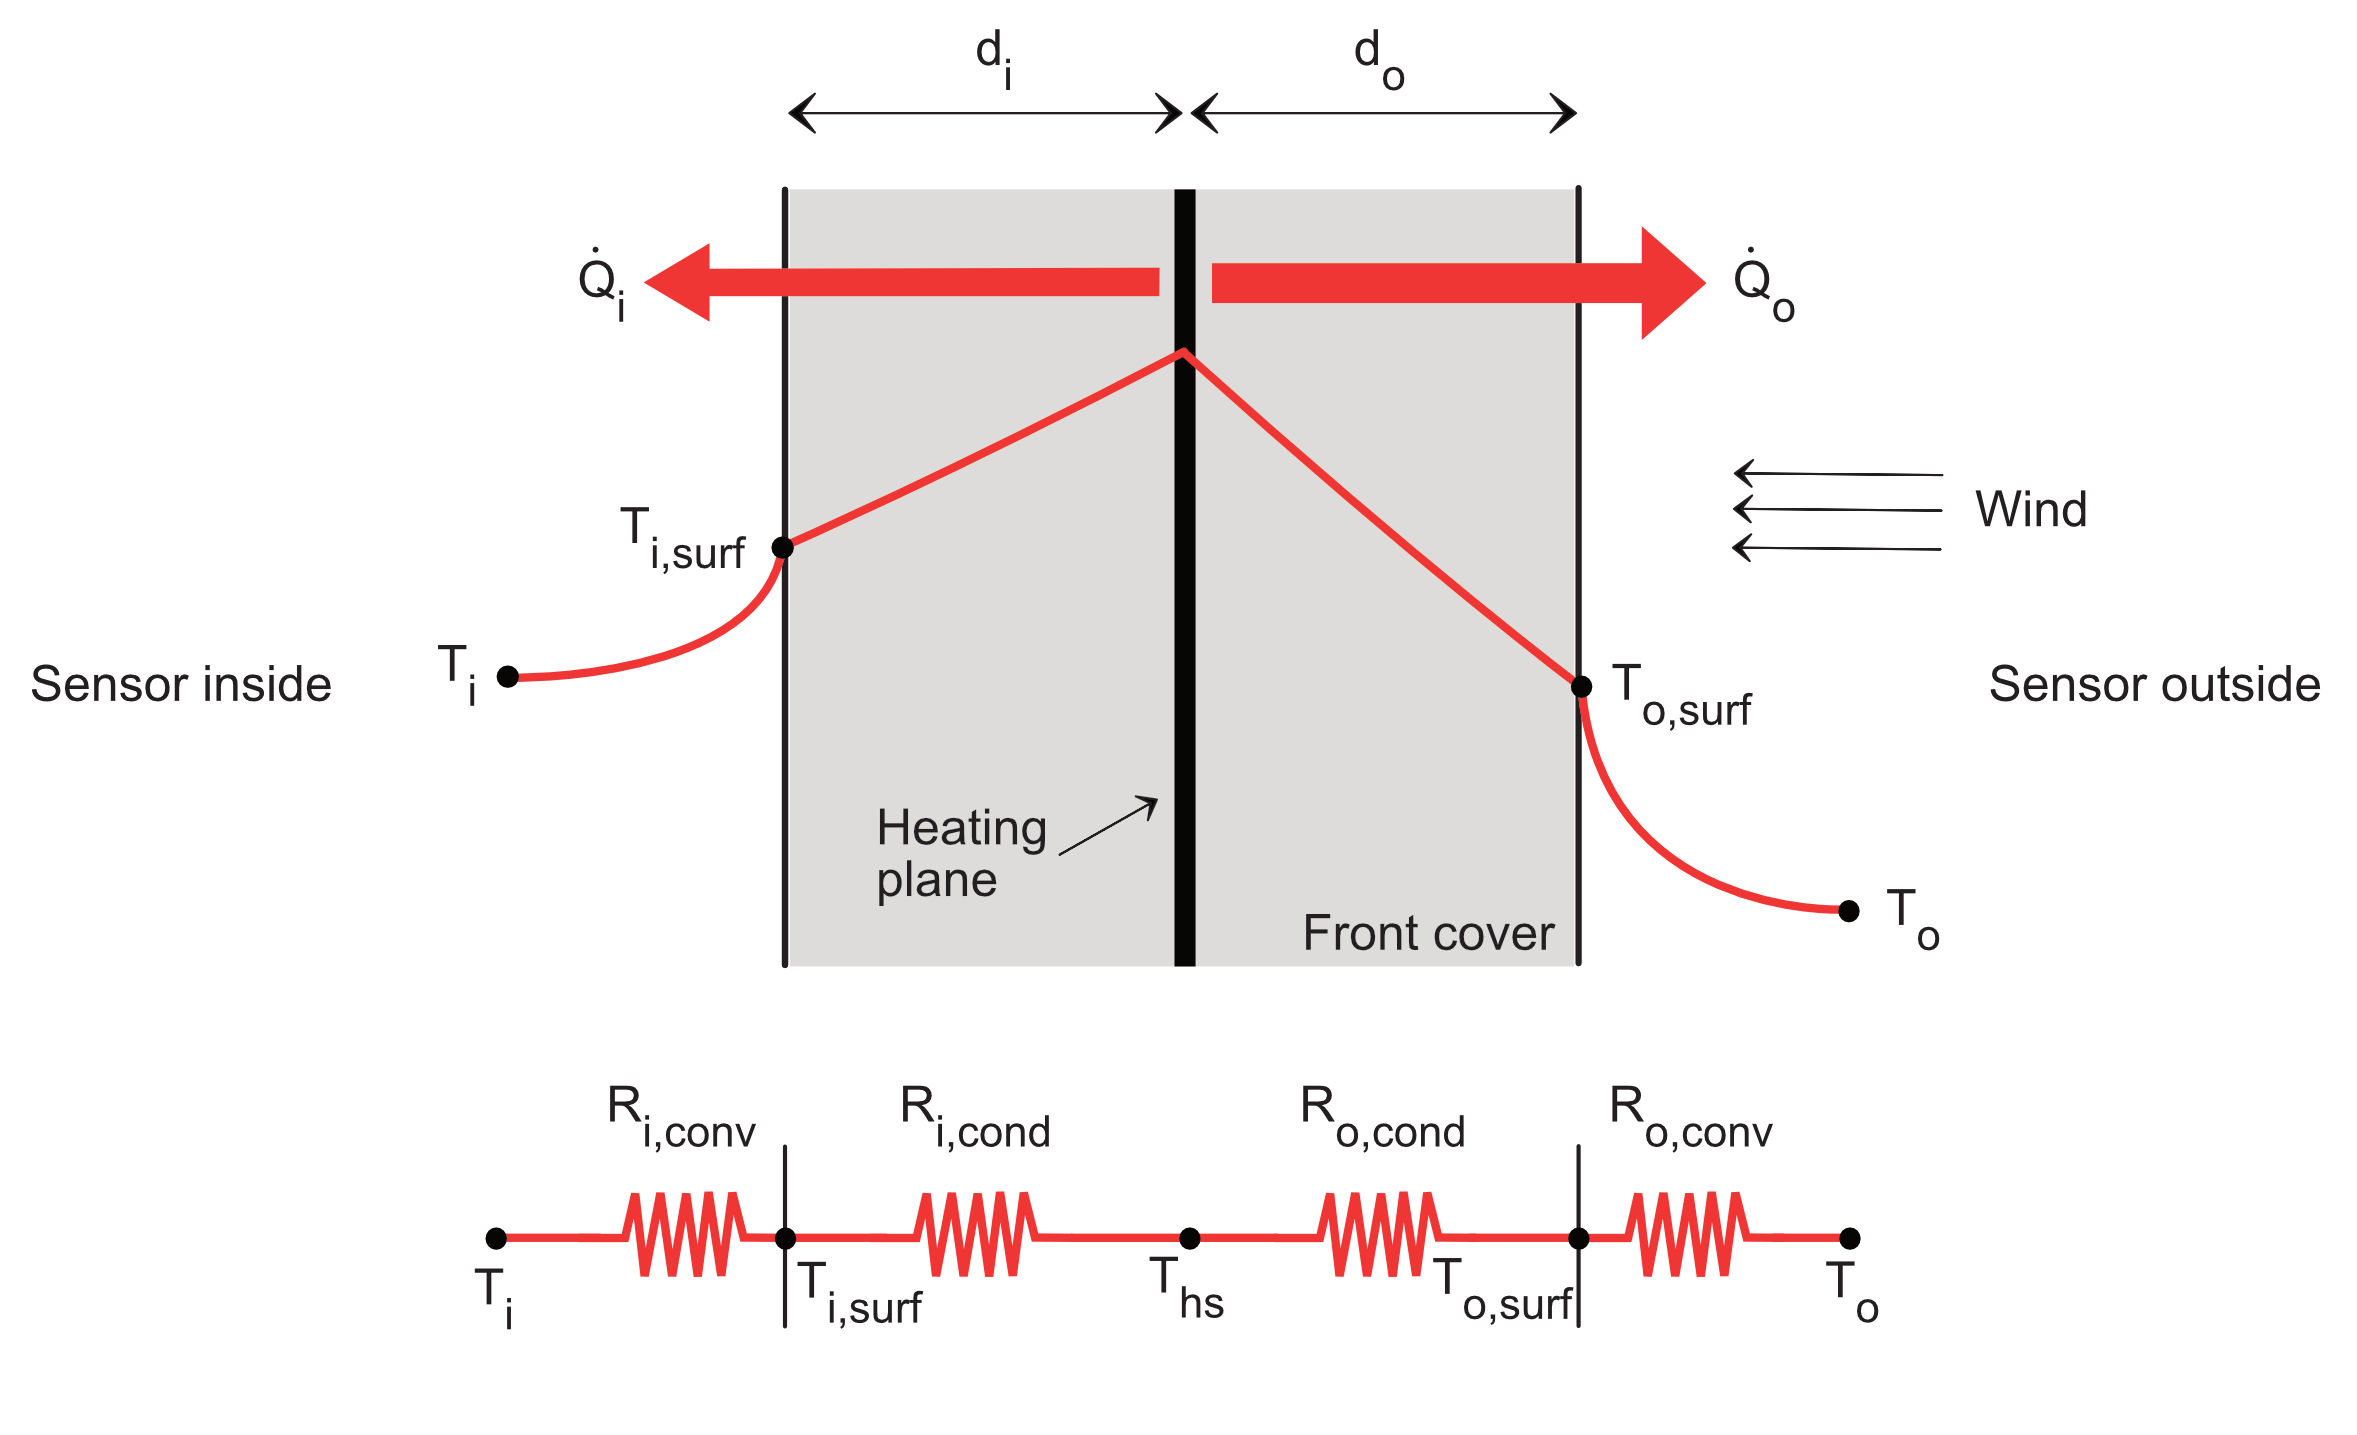
\includegraphics[scale=0.375]{\pathPics/Model.png}
	\caption[Front Cover Heat Transfer Model]{Side view sketch of a front cover with a heating plate buried in the mid plane}
	\label{fig:platemodel}
\end{figure}

The relationship of equation (5) can be found by applying the thermal resistance concept. The analogous electrical circuit is shown in the lower part of Fig. \ref{fig:platemodel}. In steady state conditions, the heat transfer rate from the heated plate to the outside is constant. Therefore, the heat transferred by conduction from the heating plate to the outer surface is exactly equal to the convection heat transfer rate from the outer surface to the ambient:
%%%%\begin{align}
%%%%\frac{\dot Q_o^{cond}}{A_h} = \frac{1}{R_o^{cond}}\cdot (T_{hs}-T_o^{surf}) \;\; &= \;\;\frac{\dot Q_o^{conv}}{A_h} = \frac{1}{R_o^{conv}}\cdot (T_o^{surf}-T_{o})
%%%%\end{align}
\begin{multline}
\frac{\dot Q_o^{cond}}{A_h} = \frac{1}{R_o^{cond}}\cdot (T_{hs}-T_o^{surf}) \;\; \\
= \;\;\frac{\dot Q_o^{conv}}{A_h} = \frac{1}{R_o^{conv}}\cdot (T_o^{surf}-T_{o})
\end{multline}
The conduction heat transfer rate per unit area \(\dot Q_o^{cond}/A_h\) is proportional to the difference between the heating plate temperature and the outer surface temperature, where \(R_o^{cond} = d_o/(\lambda A_h)\) is the thermal resistance of the material expressed in \(m^2\cdot K/\mathrm{W}\). The convection heat transfer rate per unit area \(\dot Q_o^{conv}/A_h\) is proportional to the temperature difference between the outer surface temperature and the ambient temperature. Comparing both rates leads to an expression for the surface temperature $T_o^{surf}$. It depends on the ambient temperature $T_o$, the heating plate temperature $T_{hs}$, the material parameters and the convective thermal resistance  which is determined by the wind condition:
%%%%\begin{align}
%%%%T_o^{surf}(T_o,T_{hs},\nu) \;\;\;\;\; &= \;\;\;\;\; \frac{R_o^{conv}(\nu)}{R_{o}(\nu)}\cdot T_{hs} + (1-\frac{R_o^{conv}(\nu)}{R_{o}(\nu)})\cdot T_o
%%%%\end{align}
\begin{multline}
T_o^{surf}(T_o,T_{hs},\nu) \;\;\;\;\; = \;\;\;\;\; \frac{R_o^{conv}(\nu)}{R_{o}(\nu)}\cdot T_{hs} \\
+ (1-\frac{R_o^{conv}(\nu)}{R_{o}(\nu)})\cdot T_o
\end{multline}
Here, $R_o(\nu) = R_o^{cond} + R_o^{conv}(\nu)$. The relationship between \(R_o^{conv}\) and the wind speed \(\nu\) is described in chapter \ref{chapter:windspeedrelation}. 

The relationship in equation (6) also can be found by referring to the circuit model in the lower part of Fig. \ref{fig:platemodel}. One possible way is to derive the heat transfer from the heating plate to the outer ambient \((T_{hs}-T_0)/R_o\). The heat transfer rate is a sum of two terms. The first term is the heat transfer occurs through two contributions. The first originates from heat transferred from the warmer inside to the outside. The transfer rate is equal to \((T_i - T_o)/R_{tot}\), where \(R_{tot} = R_o + R_i\) with \(R_i = R_i^{cond} + R_i^{conv}\). The second from the part of the heat that is transferred from the heating plate to the outside. The total heat emitted by the heating source is equal to the electrical power. Only a fraction is transmitted to the outer ambient. When \(R_{tot}\) is the total thermal resistance between the inside and the outside, only the fraction of \(R_i/R_{tot}\) is transferred to the outside. Therefore, expression for the total heat transfer between the heating plate to the outside amounts to
%%%%\begin{align}
%%%%\frac{T_{hs}-T_0}{R_o} \;\; &= \;\; \frac{1}{R_{tot}}\cdot (T_i - T_o)\; + \;\frac{R_i}{R_{tot}}\cdot \frac{P}{A}  \;\; = \;\; \frac{T_o^{surf}-T_o}{R_o^{conv}}
%%%%\end{align}
\begin{multline}
\frac{T_{hs}-T_0}{R_o} \;\; = \;\; \frac{1}{R_{tot}}\cdot (T_i - T_o)\; + \;\frac{R_i}{R_{tot}}\cdot \frac{P}{A}  \;\; \\
= \;\; \frac{T_o^{surf}-T_o}{R_o^{conv}}
\end{multline}
The equation can be solved for \(T_{hs}\):
%%%%\begin{align}
%%%%T_{hs}(P,T_o,T_i,\nu) \;\; &= \;\; T_o + \frac{R_o(\nu)}{R_{tot}(\nu)}\cdot (T_i - T_o) + \frac{R_o(\nu)R_i}{R_{tot}(\nu)}\cdot \frac{P}{A_h}
%%%%\end{align}
\begin{multline}
T_{hs}(P,T_o,T_i,\nu) \;\; = \;\; T_o + \frac{R_o(\nu)}{R_{tot}(\nu)}\cdot (T_i - T_o) \\
+ \frac{R_o(\nu)R_i}{R_{tot}(\nu)}\cdot \frac{P}{A_h}
\end{multline}
The heat transfer from the heating plate to the outside is the same as the heat transfer through the outer surface, which is reflected in the right expression in equation (8). This leads to the following expression for the surface temperature
%%%%\begin{align}
%%%%T_o^{surf}(P,T_o,T_i,\nu) \;\; &= \;\; T_o + \frac{R_o^{conv}(\nu)}{R_{tot}(\nu)}\cdot (T_i - T_o) + \frac{R_o^{conv}(\nu)R_i}{R_{tot}(\nu)}\cdot \frac{P}{A_h}
%%%%\end{align}
\begin{multline}
T_o^{surf}(P,T_o,T_i,\nu) \;\; = \;\; T_o + \frac{R_o^{conv}(\nu)}{R_{tot}(\nu)}\cdot (T_i - T_o) \\
+ \frac{R_o^{conv}(\nu)R_i}{R_{tot}(\nu)}\cdot \frac{P}{A_h}
\end{multline}
One of the key parameters for quantifying the heating performance is the so-called heat resistance \(\beta\) (not to mixed up with the thermal resistance \(R\)). It is a figure stating by how much the temperature increases at a certain position in the system with the heating power brought into the system. Important positions are the heating source and the surface temperature:
\begin{align}
\beta_{hs} \;\; &= \;\; \frac{\partial T_{hs}}{\partial P} \;\; = \;\; \frac{R_oR_i}{R_{tot}A_h} \\
\beta_o^{surf} \;\; &= \;\; \frac{\partial T_o^{surf}}{\partial P} \;\; = \;\; \frac{R_o^{conv}R_i}{R_{tot}A_h}
\end{align}
Both coefficients decrease with increasing wind speed. Finally, depending on the LiDAR sensor design the inner temperature \(T_i\) may increase when heating up the front cover. Then, it must be considered that the inner temperature is a function of the heating power. 

The goal of this analysis is to figure out which heating plate temperature (or heating power) is sufficient to heat up the outer surface to +5°C. The required temperature depends on the outer heat transfer coefficient, so on the wind speed, and on the ambient temperature. The temperature value can be plotted in a two-dimensional graph as shown in Fig. \ref{fig:PlateTemp} for the following material and design configuration parameters. 
\begin{center}
\begin{tabular}{||l l||} 
 \hline
 \multicolumn{2}{|c|}{Heating Plate Architecture} \\
 \hline\hline
 Parameter & Value\\
 \hline\hline
 \(d_i\) & 0 mm  \\ 
 \hline
 \(d_o\) & 4.5 mm  \\ 
 \hline
 Front Cover Thickness & 4.5 mm \\
 \hline
 Front Cover Width & 54 mm  \\ 
 \hline
 Front Cover Length & 88 mm \\
 \hline
 Front Cover Area & 47 cm²  \\
 \hline
 Thermal Conductivity & 0.7 W/m-K \\ [1ex] 
 \hline
\end{tabular}
\end{center}


\begin{figure}[ht]
\centering
\begin{minipage}[b]{0.48\linewidth}
\begin{figure} [H]
	\centering
	\includegraphics[scale=0.245]{\pathPics/Plate_Tsurf5_PlateTemp.png}
	\caption[Heating Plate - Plate Temperature Graph]{Plate temperature (°C) required to reach an outer surface temperature of +5\dC.}
	\label{fig:PlateTemp}
\end{figure}

%\caption{Happy Smiley}
%\label{fig:minipage1}
\end{minipage}
\quad
\begin{minipage}[b]{0.48\linewidth}
\begin{figure} [H]
	\centering
	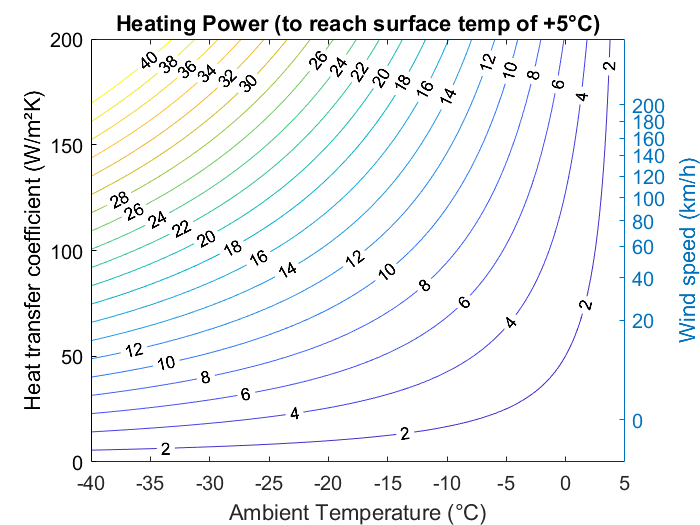
\includegraphics[scale=0.245]{\pathPics/Plate_Tsurf5_Power.png}
	\caption[Heating Plate - Heating Power Graph]{Heating power (W) required to reach a outer surface temperature of +5\dC.}
	\label{fig:PlatePower}
\end{figure}
%\caption{Sad Smiley}
%\label{fig:minipage2}
\end{minipage}
\end{figure}




\paragraph{Voltage and Duty Cycle}
Instead of expressing the heating source temperature as a function of electrical power, sometimes it is more convenient to express the surface temperature as a function of the applied voltage and the applied electrical duty cycle \(D\) of the pulse width modulation. Therefore, the power can be replaced by the following expression
\begin{align}
P \;\; &= \;\; \frac{D\cdot U^2}{R_{el}(T_{hs})}
\end{align}
with the supply voltage \(V\), the applied electrical duty cycle \(D\) of the pulse width modulation, and the electrical resistance as a function of temperature \(R_{el}(T_{hs})\). However, as the electrical resistance of the heating element depends on its temperature, also the electrical power \(P\) depends indirectly on the heating source temperature. The resistance depends on the temperature as follows:
\begin{align}
R_{el} = R_{el,20}\cdot(1 + \alpha\cdot (T_{hs}-T_{20}))
\end{align}
Here, \(\alpha\) is the temperature coefficient of electrical resistance and \(R_{el,20}\) the electrical resistance at \(T_{20} = 20^{\circ}C\). Inserting equation (12) into equation (10) leads to a quadratic equation in the heating source temperature,
\begin{align}
0 \;\; &= \;\; a\cdot T_{hs}^2 + b\cdot T_{hs} + c  
\end{align}
with a solution leading to the expression of the temperature as a function of 
\begin{align}
T_{hs}(D,U,R_{el,20},T_o,T_i,\nu) \;\; &= \;\; \frac{-b + \sqrt{b^2-4ac}}{2a}
\end{align}
with the coefficients
%%%\begin{align}
%%%a \; &= \; R_{el,20}\cdot \alpha \\
%%%b \; &= \; R_{el,20}\cdot\left(1-\alpha\cdot(T_o+T_{20}+\frac{R_o}{R_{tot}}(T_i-T_o))\right) \\
%%%c \; &= \; (\alpha\cdot T_{20}-1)\cdot\left(R_{el,20}T_o + \frac{R_{el,20}R_o}{R_{tot}}(T_i - T_o)\right) - \frac{R_oR_i}{R_{tot}A_h}\cdot D\cdot U^2
%%%\end{align}
\begin{multline}
a \; = \; R_{el,20}\cdot \alpha \\
b \; = \; R_{el,20}\cdot\left(1-\alpha\cdot(T_o+T_{20}+\frac{R_o}{R_{tot}}(T_i-T_o))\right) \\
c \; = \; (\alpha\cdot T_{20}-1)\cdot\left(R_{el,20}T_o + \frac{R_{el,20}R_o}{R_{tot}}(T_i - T_o)\right) \\
- \frac{R_oR_i}{R_{tot}A_h}\cdot D\cdot U^2
\end{multline}


\begin{itemize}
\item Shape Factor
\item NEXT Makrolon Picture
\item NEXT Glass Picture
\item NEXT Glass Formula Plot
\end{itemize}

\subsection{Relationship between Heat Transfer Coefficient and Wind Speed}\label{chapter:windspeedrelation}
The thermal resistance for convection is typically defined as the inverse of the heat transfer coefficient \(h_o^{conv} = 1/R_o^{conv}\) expressed in \(\mathrm{W}/m^2\cdot K\). The following table lists typical values of the heat transfer coefficient for different type of convection \cite{Unnamed-2}: 

\begin{table} [H]
\centering
\color{B}
\begin{tabular} [h] {  p{50mm} p{27mm} }
Type of convection & $h, \unit{W/{m^2\cdot K}}$ \\ \hline
Natural convection of gases & 2 - 25 \\ 
Forced convection of gases & 10 - 250 
\end{tabular}
%\caption[Heat transfer coefficient of gases]{List of typical values for different heat transfer coefficients.}
%\label{tab:HTC}
\end{table}
The relationship between the heat transfer coefficient and the wind speed depends on the exact inflow and is therefore not easy to be calculated for the real system. The heat transfer coefficient for a low speed flow of air over a surface is about \(h_o^{conv} = 20 \,\,\,\unit{W/m^2\cdot K}\). Low speed means speeds of around $1 \unit{km/h}$. This value gives well matching simulation results when comparing to experimental data recorded with the NEXT LiDAR sensor front cover. For higher wind speeds the following relation is the best fit to a series of data points shown in Fig. \ref{fig:HTC}: 
\begin{equation}
h_o^{conv} = h_0 + a\cdot \sqrt{v}
\end{equation}
with \(a = 20 \, \,\mathrm{W\cdot s^{1/2}/(K\cdot m^{5/2})}\) and the wind speed $v$ is given in m/s. 
Figure \ref{fig:HTC} shows experimental data points in blue with a fitting curve given by equation (21). 
\begin{figure} [H]
	\centering
	\includegraphics[scale=0.3]{\pathPics/htc-v.png}
	\caption[Heat Transfer Coefficient vs Wind Speed]{Estimated heat transfer coefficient for the front cover outer surface of the NEXT 1T LiDAR sensor (in the B1 development phase) as a function of the wind speed. The plot shows the best fit (blue curve) to the series of data points from experiment and simulation (red dots).}
	\label{fig:HTC}
\end{figure}


%\begin{figure} [H]
%	\centering
%	\includegraphics[scale=0.5]{Pictures/Plate_Tsurf5_PlateTemp.png}
%	\caption[Front Cover Heat Transfer Model]{Side view sketch of a front cover with a heating plate buried in the mid plane}
%	\label{fig:fig1}
%\end{figure}
%
%\begin{figure} [H]
%	\centering
%	\includegraphics[scale=0.5]{Pictures/Plate_Tsurf5_Power2.png}
%	\caption[Front Cover Heat Transfer Model]{Side view sketch of a front cover with a heating plate buried in the mid plane}
%	\label{fig:fig1}
%\end{figure}

\subsection{Heating Wire Architecture}
The shape factor is defined to be \cite{1975EHahne_UG}
\begin{align}
P \;\; &= \;\; \lambda \cdot S \cdot \Delta T
\end{align}
For a wall, the shape factor is then
\begin{align}
S \;\; = \;\; \frac{A}{d}
\end{align}
For complex geometries it must be found. For heating wire embedded in the front cover the following formula can be used
\begin{align}
S \;\; = \;\; \frac{N\cdot 2pi\cdot L}{\log\left(\frac{4w}{\pi\cdot z}\cdot sinh(2\pi \cdot d/w)\right)} \;\; = \;\; 0.6 \mathrm{m}
\end{align}
with \(N = 14\) the number of wires, L the width of the heating area, \(z\) the diameter of the heating wires, \(w\) the wire pitch and \(d\) the thickness between the wire plane and the surface.
\begin{figure} [H]
	\centering
	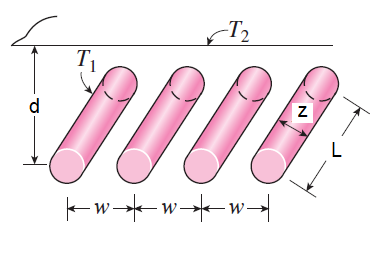
\includegraphics[scale=0.4]{\pathPics/TheoryShapeFactorMakrolon.png}
	\caption[NEXT LiDAR Sensor Model]{ddd}
	\label{fig:ShapeFactorMakrolon}
\end{figure}
\section{PDE Simulation}
\section{Front Cover Heating of the NEXT LiDAR Sensor}

\begin{figure} [H]
	\centering
	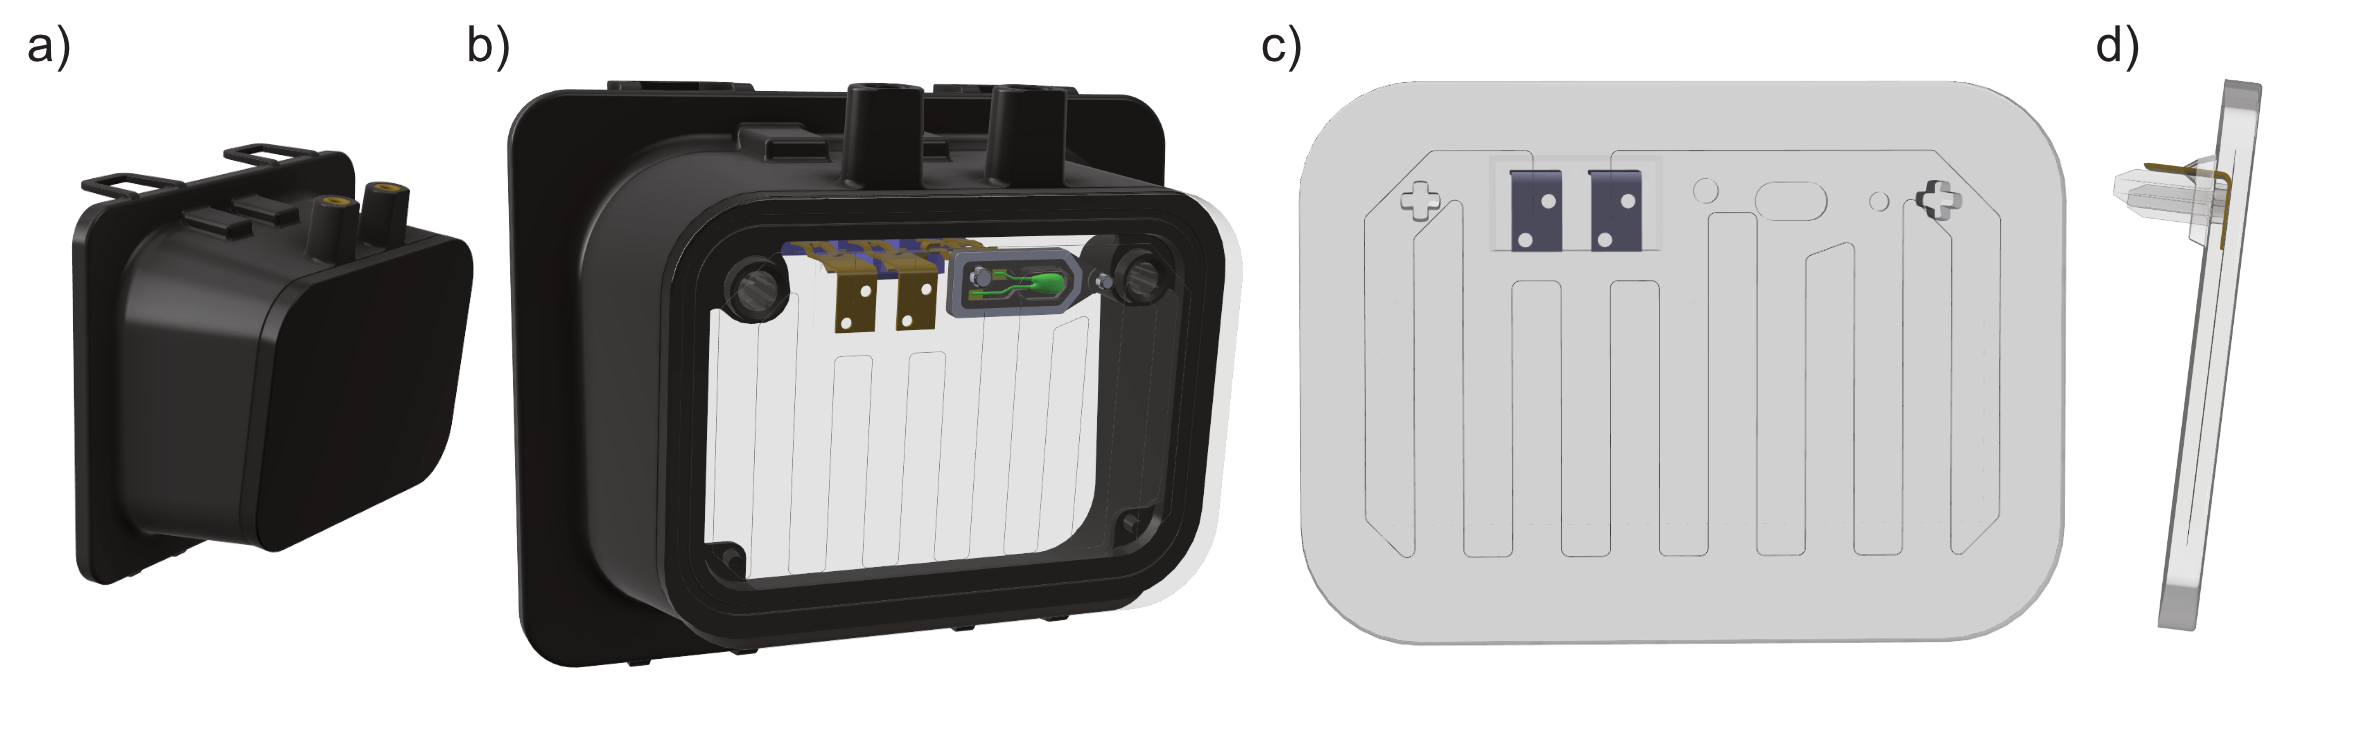
\includegraphics[scale=0.4]{\pathPics/1TB1_3DModel.png}
	\caption[NEXT LiDAR Sensor Model]{ddd}
	\label{fig:1TB1Model}
\end{figure}


\begin{figure}[ht]
\centering
\begin{minipage}[b]{0.48\linewidth}
\begin{figure} [H]
	\centering
	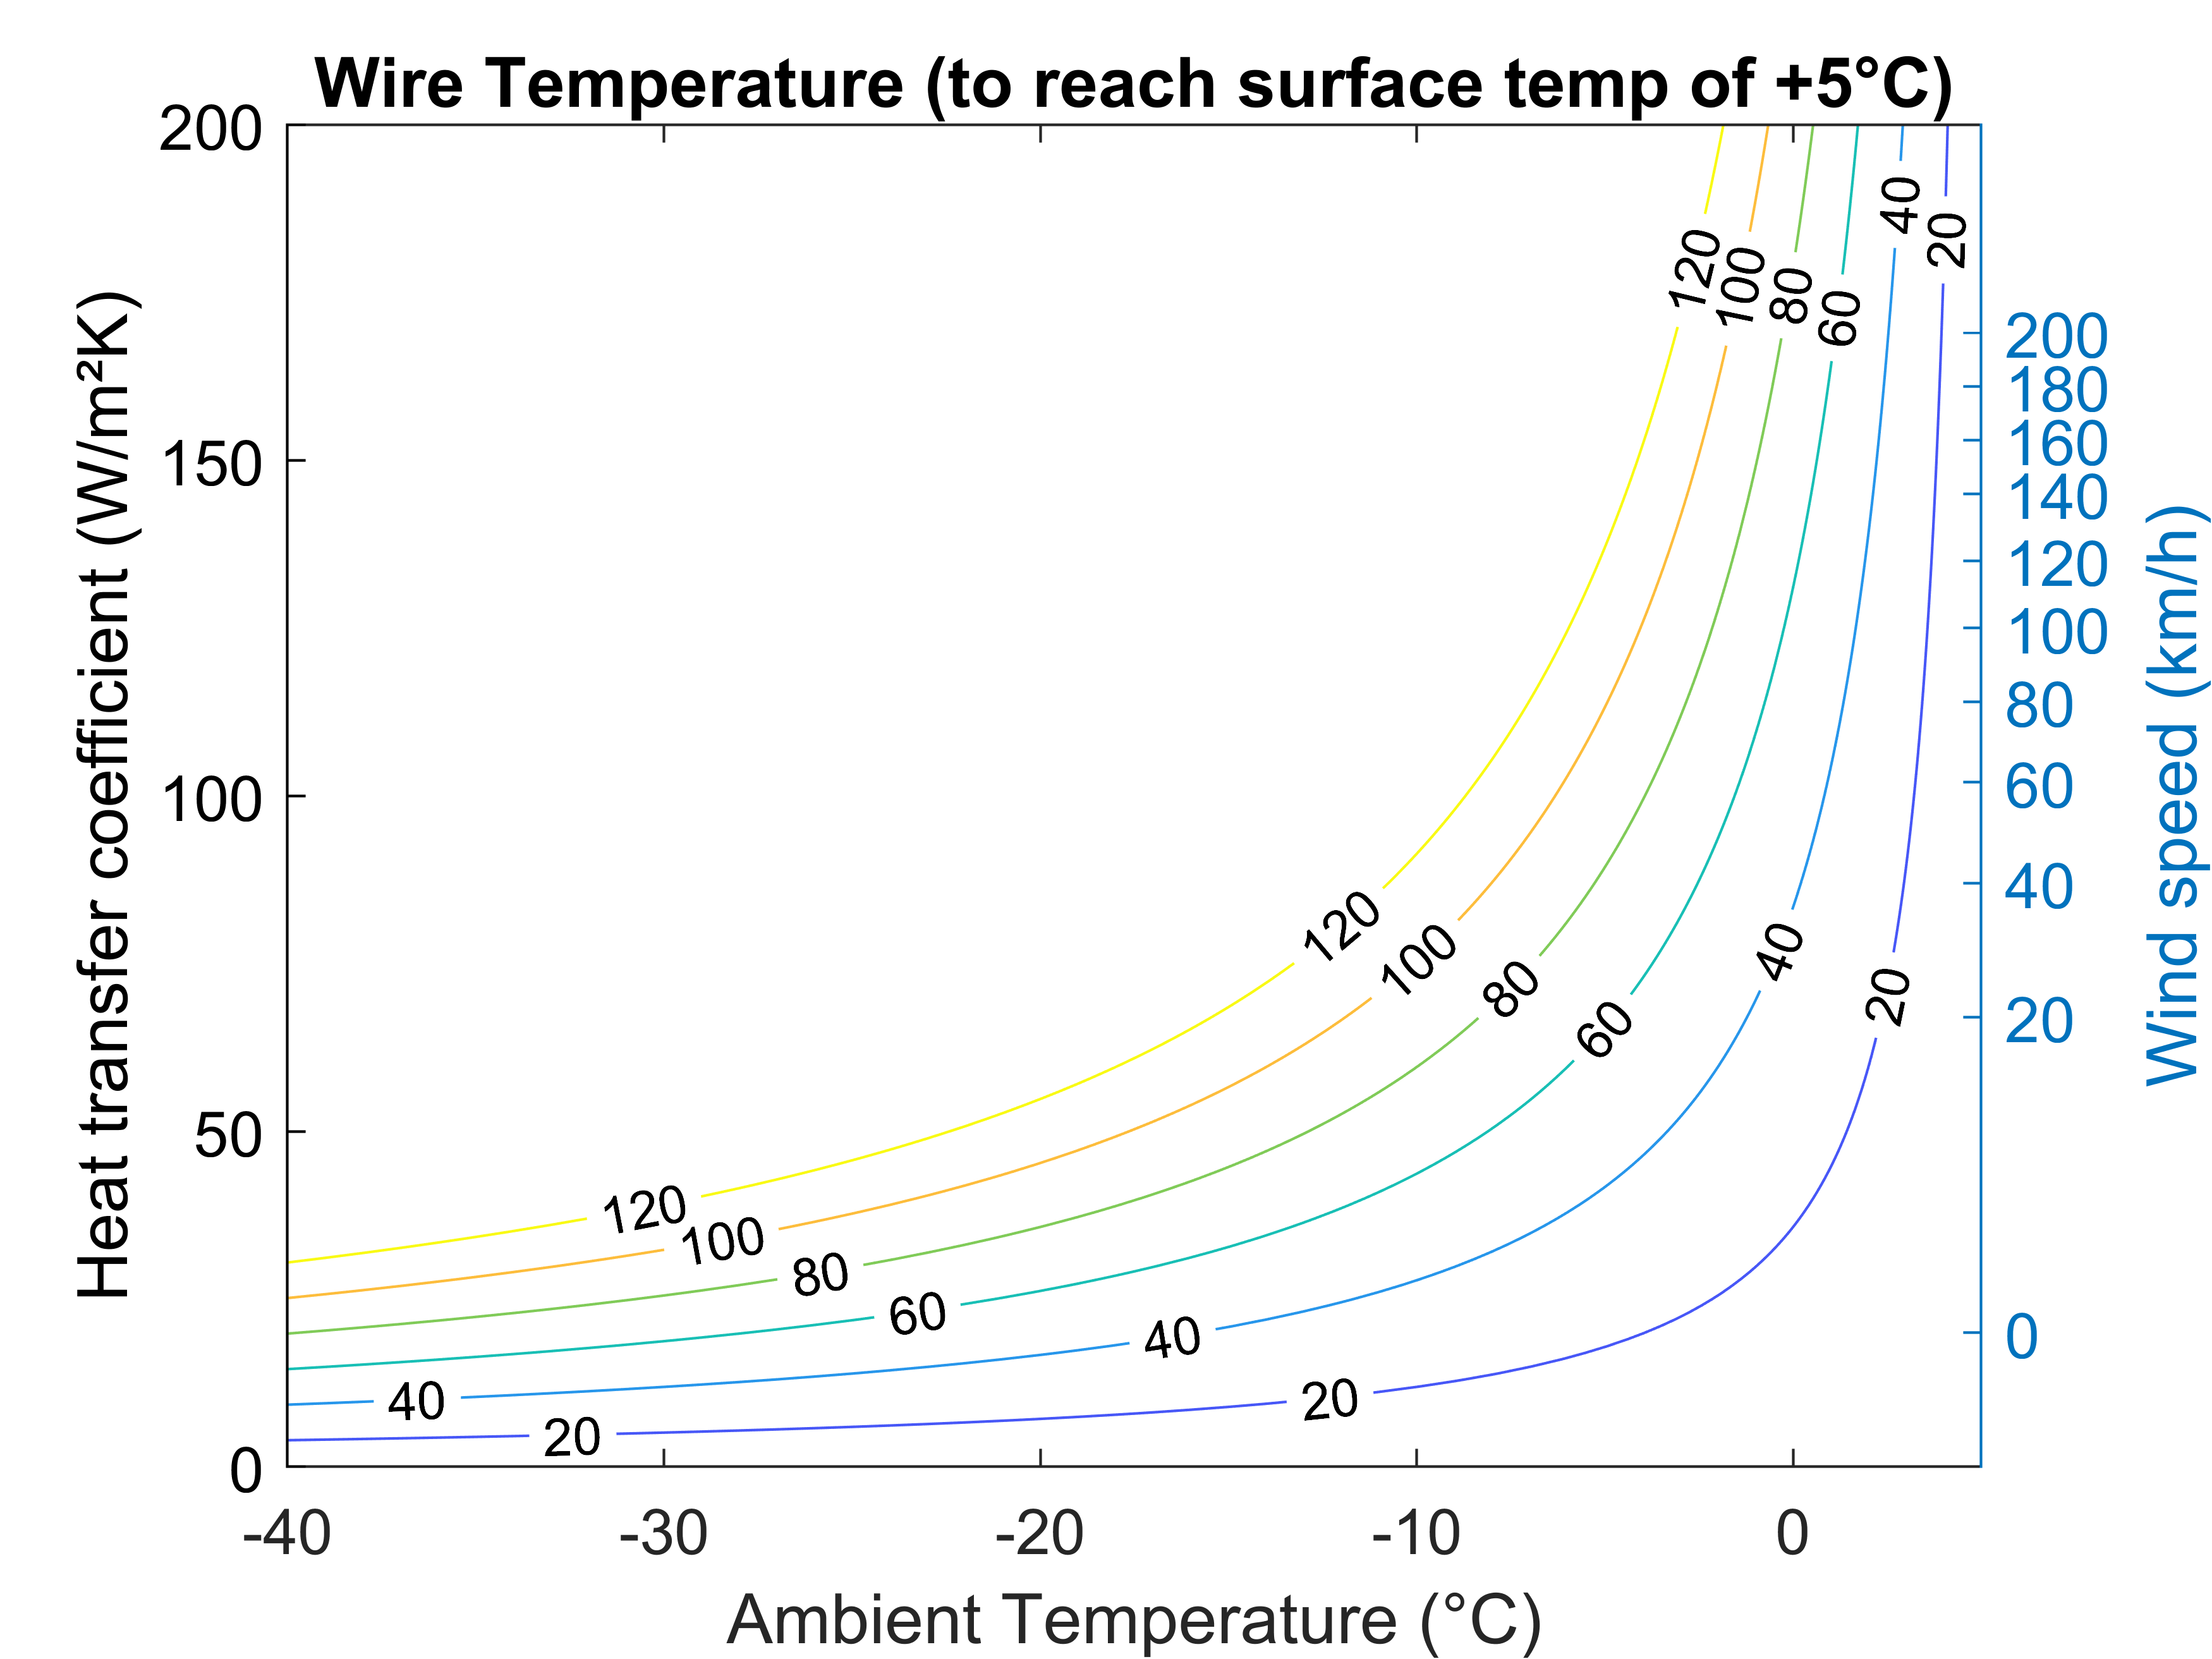
\includegraphics[scale=0.245]{\pathPics/B1Glass_Tsurf5_WireTemp.png}
	\caption[Front Cover Heat Transfer Model]{Side view sketch of a front cover with a heating plate buried in the mid plane }
	%\label{fig:fig1}
\end{figure}

%\caption{Happy Smiley}
%\label{fig:minipage1}
\end{minipage}
\quad
\begin{minipage}[b]{0.48\linewidth}
\begin{figure} [H]
	\centering
	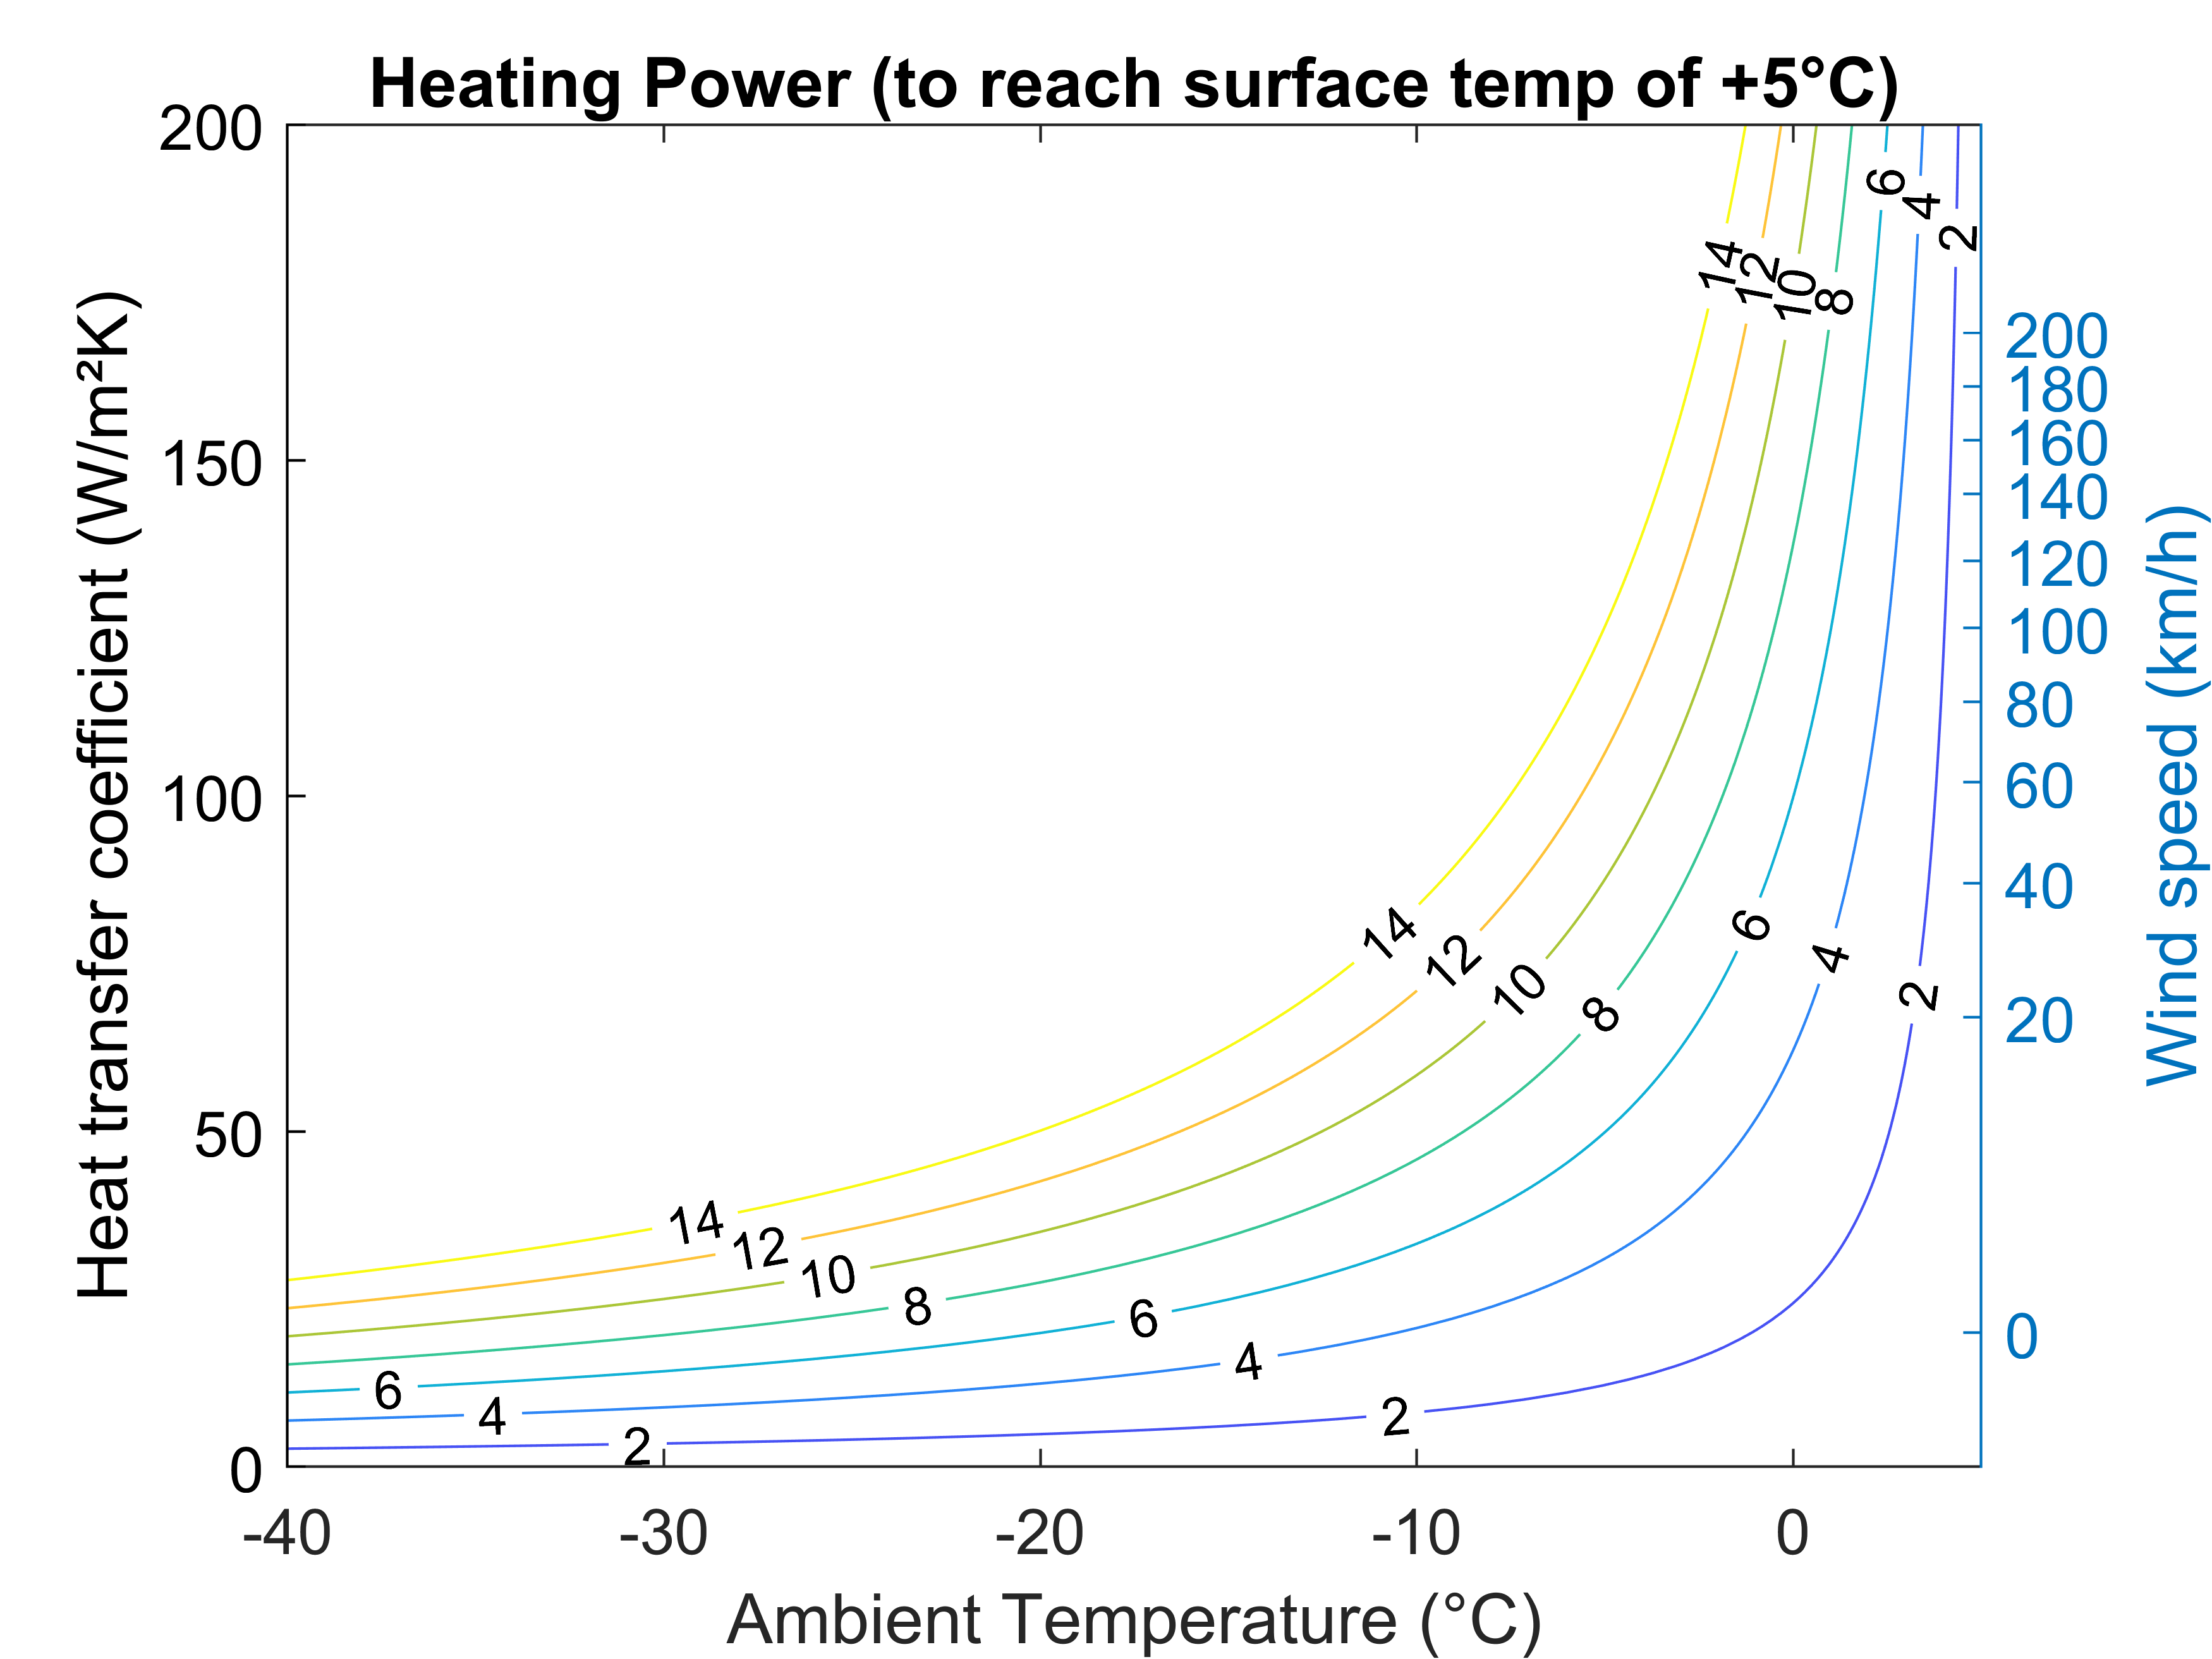
\includegraphics[scale=0.245]{\pathPics/B1Glass_Tsurf5_Power.png}
	\caption[Front Cover Heat Transfer Model]{Side view sketch of a front cover with a heating plate buried in the mid plane}
	%\label{fig:fig1}
\end{figure}
%\caption{Sad Smiley}
%\label{fig:minipage2}
\end{minipage}
\end{figure}


\begin{figure}[ht]
\centering
\begin{minipage}[b]{0.48\linewidth}
\begin{figure} [H]
	\centering
	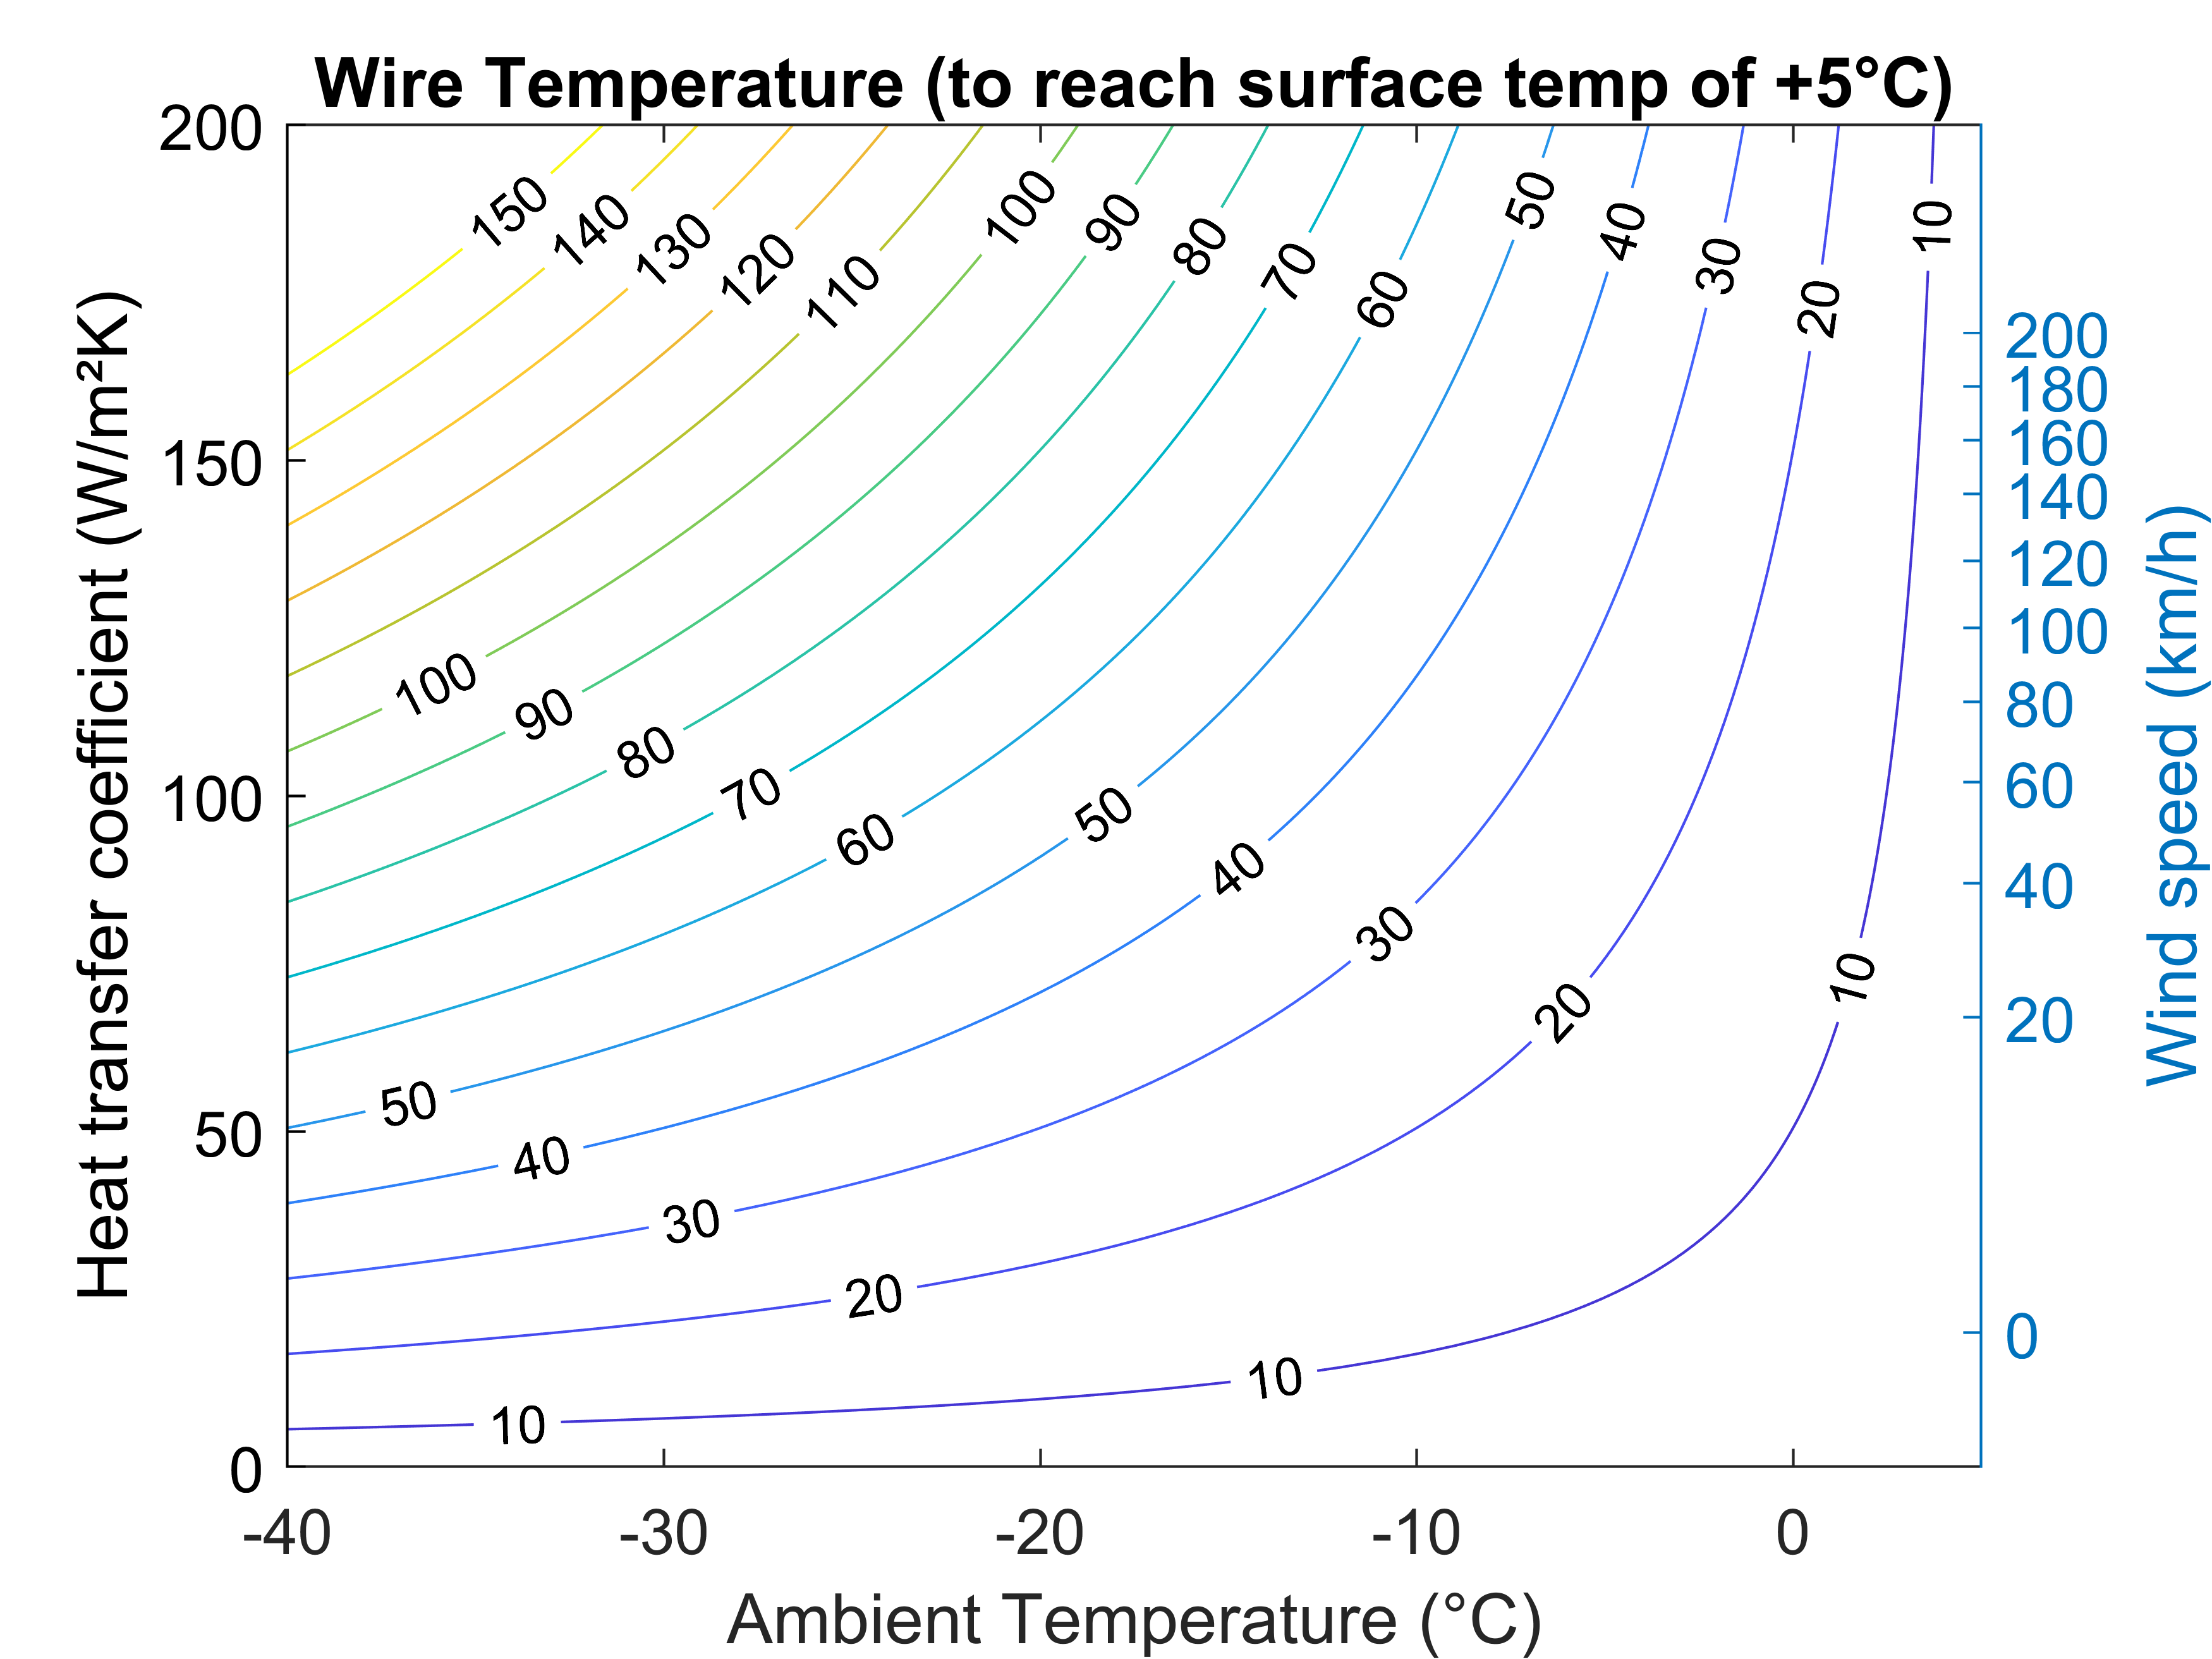
\includegraphics[scale=0.255]{\pathPics/B1Makrolon_Tsurf5_WireTemp.png}
	\caption[Front Cover Heat Transfer Model]{Side view sketch of a front cover with a heating plate buried in the mid plane }
	%\label{fig:fig1}
\end{figure}

%\caption{Happy Smiley}
%\label{fig:minipage1}
\end{minipage}
\quad
\begin{minipage}[b]{0.48\linewidth}
\begin{figure} [H]
	\centering
	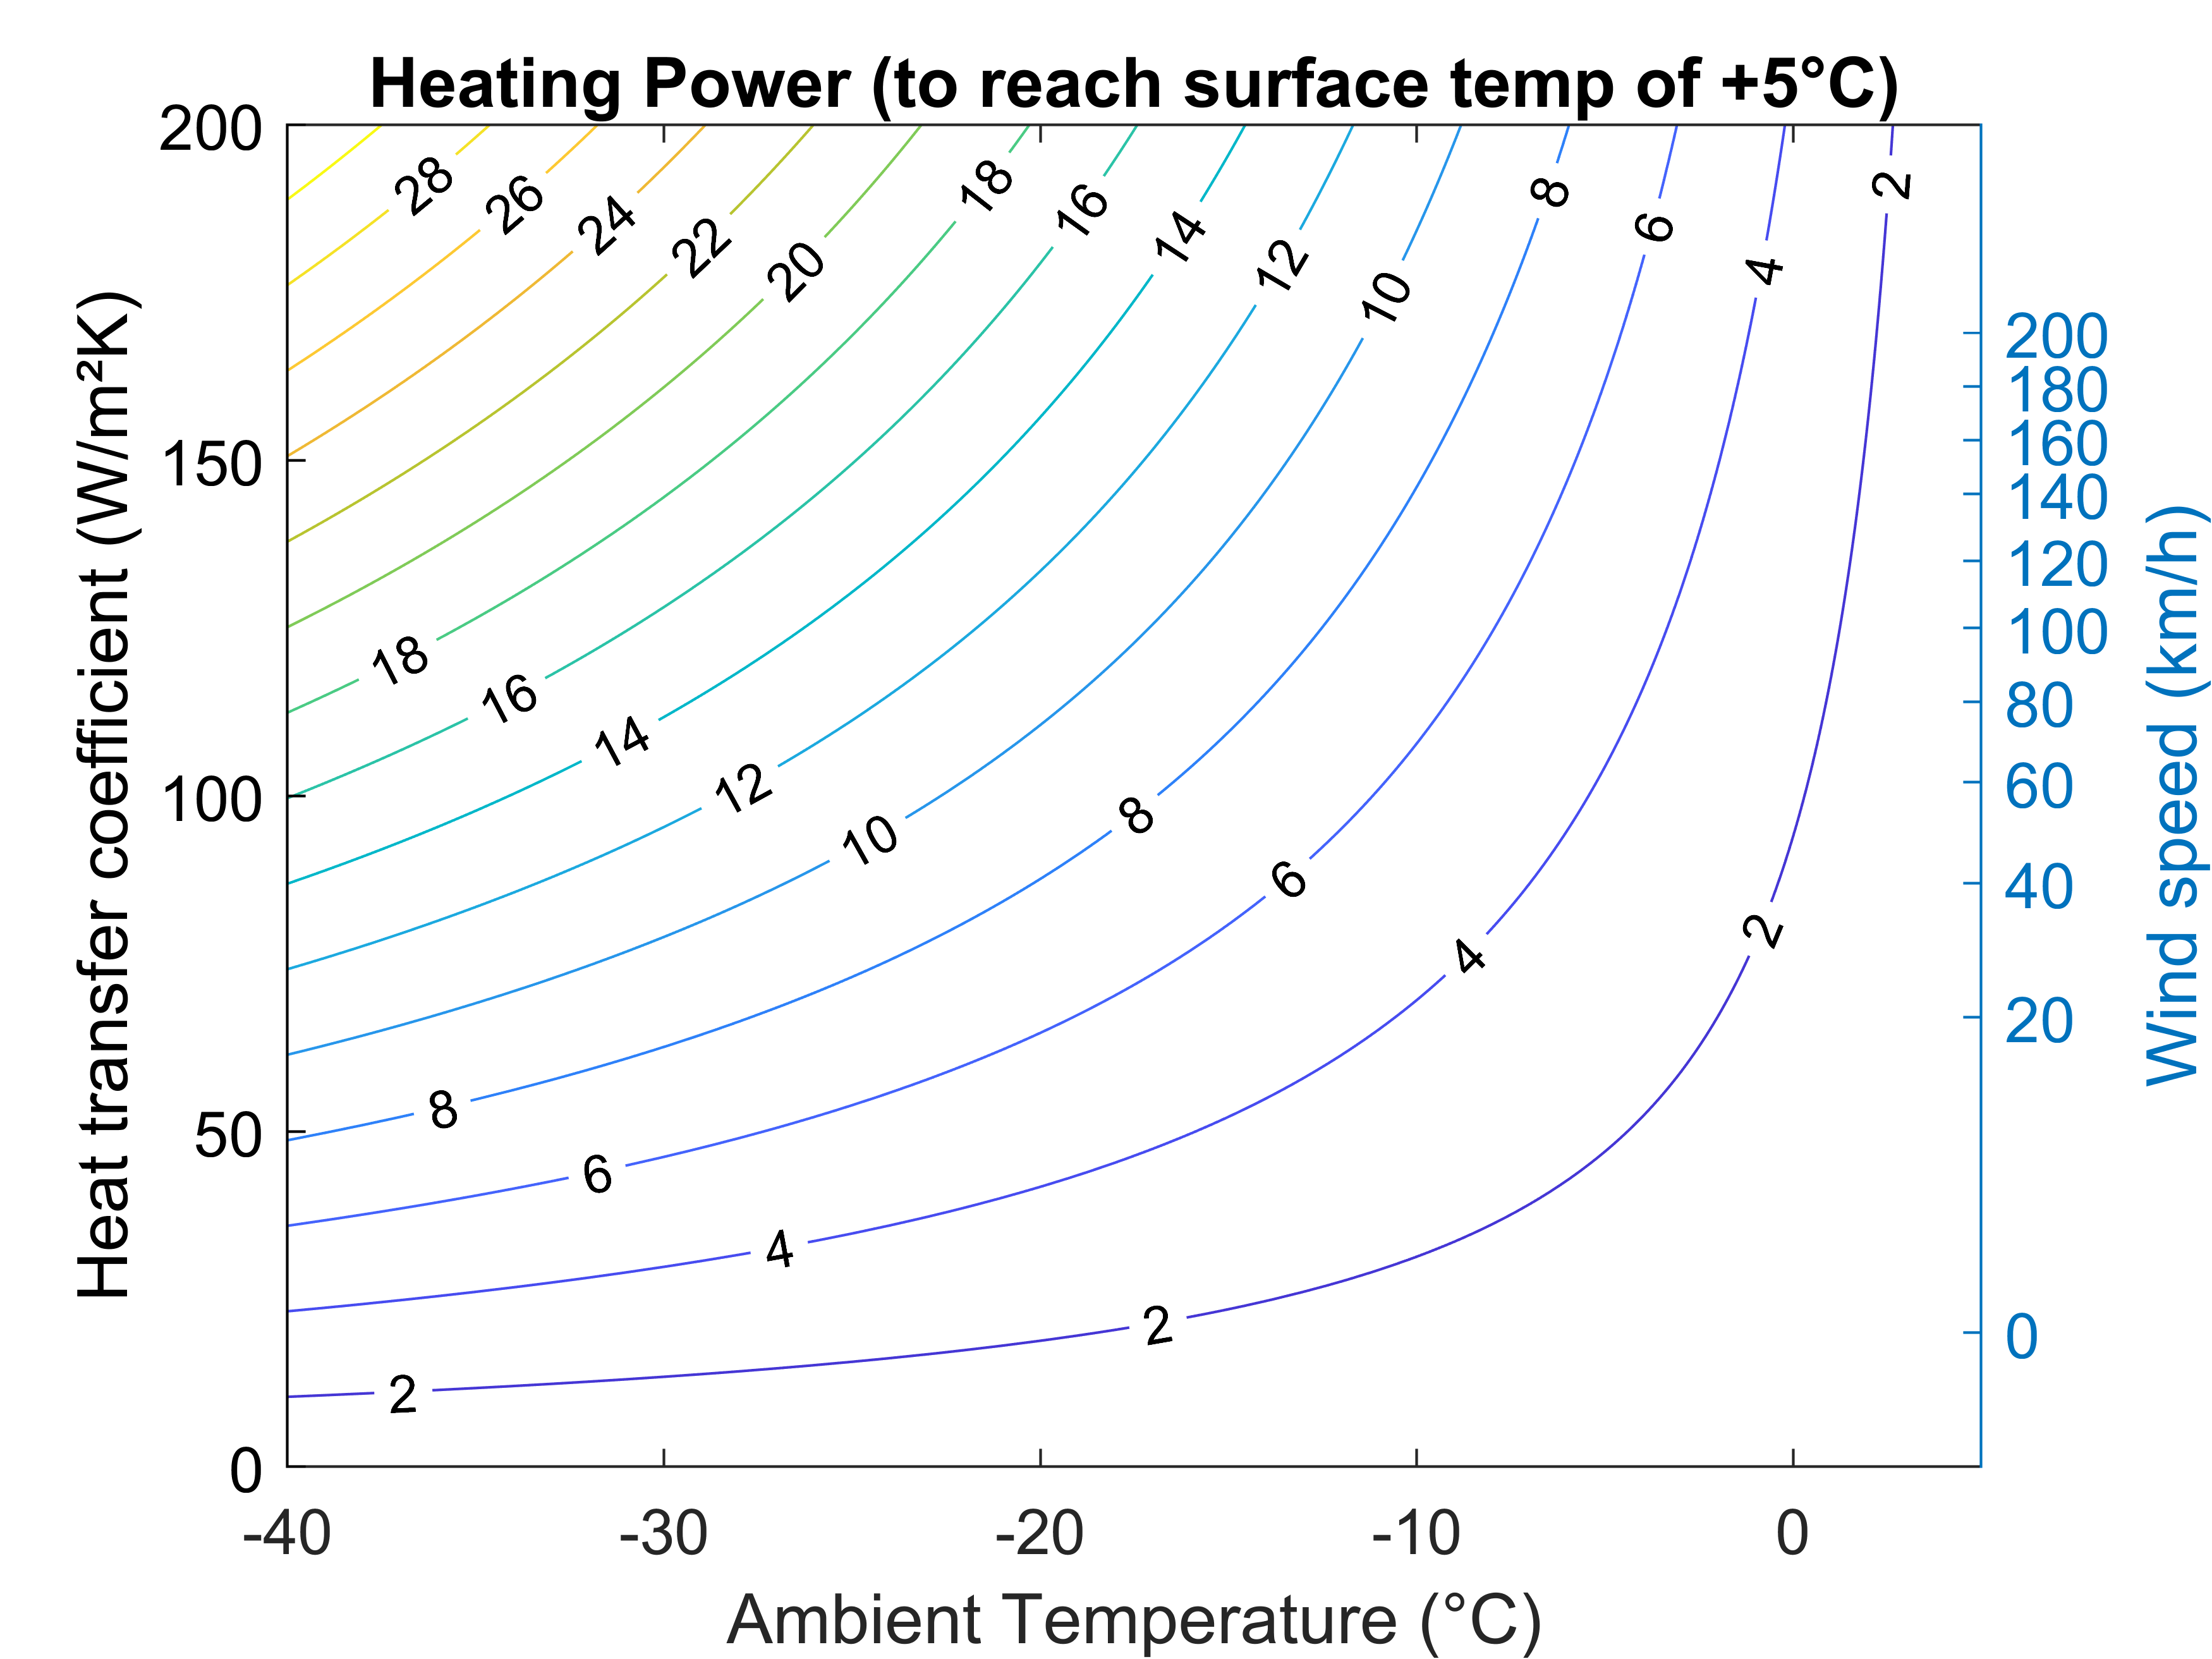
\includegraphics[scale=0.255]{\pathPics/B1Makrolon_Tsurf5_Power.png}
	\caption[Front Cover Heat Transfer Model]{Side view sketch of a front cover with a heating plate buried in the mid plane}
	%\label{fig:fig1}
\end{figure}
%\caption{Sad Smiley}
%\label{fig:minipage2}
\end{minipage}
\end{figure}

%TEXT
 

%\begin{table} [H]
%\color{B}
%\begin{tabular} [h] {p{30mm} | p{27mm} | p{27mm} | p{27mm} | p{27mm} }
%\rowcolor{LG}
% &  & & &  \\ \hlineRed
% &  &  &  & \\ \hline
% &  &  &  & \\
%\end{tabular}
%\caption[Name of an example table]{Name of an example table. Long text...}
%\label{tab:tab1}
%\end{table}

%\section{Key Performance Indicators}
%In this chapter, key figures are listed that should either be defined ....


%The surface temperature $T_o$ can be expressed as a function of the setpoint temperature, ambient temperature and the heating transfer coefficients:
%\begin{eqnarray}
%T_o^{surf} = a(R_o)\cdot T_{hs} + b(R_o)\cdot T_o \\
%a(R_o) = \frac{R_o^{conv}}{R_o} \\
%b(R_o) = 1-\frac{R_o^{conv}}{R_o}
%\end{eqnarray}


%The total heat transfer rate per unit area \(\dot Q_{tot}/A_h\), or heating power \(P/A_h\) per unit area, is equal to the heat flux through the frontside \(\dot Q_o/A_h\) plus the heat flux through the backside \(\dot Q_i/A_h\) of the frontcover, where $A_h$ is the area through with the heat transfer takes place. 
%The analogous electric circuit of the heating plate architecture is shown on the lower part of Fig. 2. 
%\begin{equation}
%\frac{P}{A} = \frac{\dot Q_o}{A_h} + \frac{\dot Q_i}{A_h} = \frac{1}{R_{i}}\cdot (T_{hs} - T_{i}) + \frac{1}{R_o}\cdot (T_{hs} - T_{o})
%\end{equation}
%
%Equation (1) can be expressed in another form
%\begin{equation}
%\frac{P}{A} = \frac{R_{tot}}{R_{o} R_{i}}\cdot(T_{hs}-T_{o}) - \frac{1}{R_{i}}\cdot(T_{i}-T_{o})
%\end{equation}
%The dissipated power per unit area ... Equation (4) consists of two terms: If the 
%By rearranging equation (1), the temperature of the heating plate can be found to be 
%\begin{equation}
%T_{hs} = \frac{R_{o} R_{i}}{R_{tot}}\cdot\frac{P}{A} + \frac{R_{o}}{R_{tot}}\cdot(T_{i}-T_{o}) + T_{o} 
%\end{equation}
%with the total resistance of the front cover $R_{tot} = R_i + R_o$. Inserting $T_{hs}$ into equation (2) results in the expression for the surface temperature as a function of the heating power $P$, the ambient temperature $T_o$ and the heat transfer coefficient $h_o^{conv}$, which depends on the wind speed:
%\begin{equation}
%T_o^{surf} = T_o + \frac{R_o^{conv}}{R_o}\cdot(\frac{R_{o} R_{i}}{R_{tot}}\cdot\frac{P}{A} + \frac{R_{o}}{R_{tot}}\cdot(T_{i}-T_{o}))
%\end{equation}
%\begin{equation}
%T_o^{surf} = T_o + \frac{R_o^{conv} R_{i}}{R_{tot}}\cdot\frac{P}{A} + \frac{R_o^{conv}}{R_{tot}}\cdot(T_{i}-T_{o})
%\end{equation}


%with $d_o$ the distance between the heating plate and the surface and $k$ the thermal conductivity of the material


%\begin{mdframed}[style=MyFrame]
%\begin{align}
%R_{tot} &=  R_{o}+ R_{i} \\
%R_{o} &=  R_o^{cond}+ R_o^{conv} \\
%R_{i} &=  R_i^{cond}+ R_i^{conv}
%\end{align}
%
%\end{mdframed}

%!TEX root = 0_document_de.tex
\section{Appendix}
\subsection{Passive Front Cover Heating}
To defrost ice accumulated on the outer surface of the LiDAR sensor without an active heating element, warm air need to be blown over the inner surface of the front cover, in the same way as an automobile windshield is defrosted. The air within a closed sensor is only weakly circulating though, with a wind speed of less than 1 km/h. Consider a front cover with a thickness of $d = 4 \unit{mm}$ and thermal conductivity of \(k = 1 \,\, \unit{W/m\cdot K}\). The outside ambient temperature is \(T_{amb} = -5\dC\) and the convection heat transfer coefficient is \(h_{out} = 25 \, \, \unit{W/m²\textbullet K}$, which corresponds to a front cover exposed to a wind speed of about 1 km/h. Also consider a sensor with a front cover area of 45 \unit{cm^2} and an average power consumption of 5 \unit{W}. As shown in the following, the outer front cover surface is not heated up to the melting point. Even when increasing the power consumption and using a thinner front cover, the passive heating is not sufficient to cause the accumulated ice to begin melting if the surface is exposed to slightly higher wind speeds or lower ambient temperatures.


\begin{figure} [H]
	\centering
	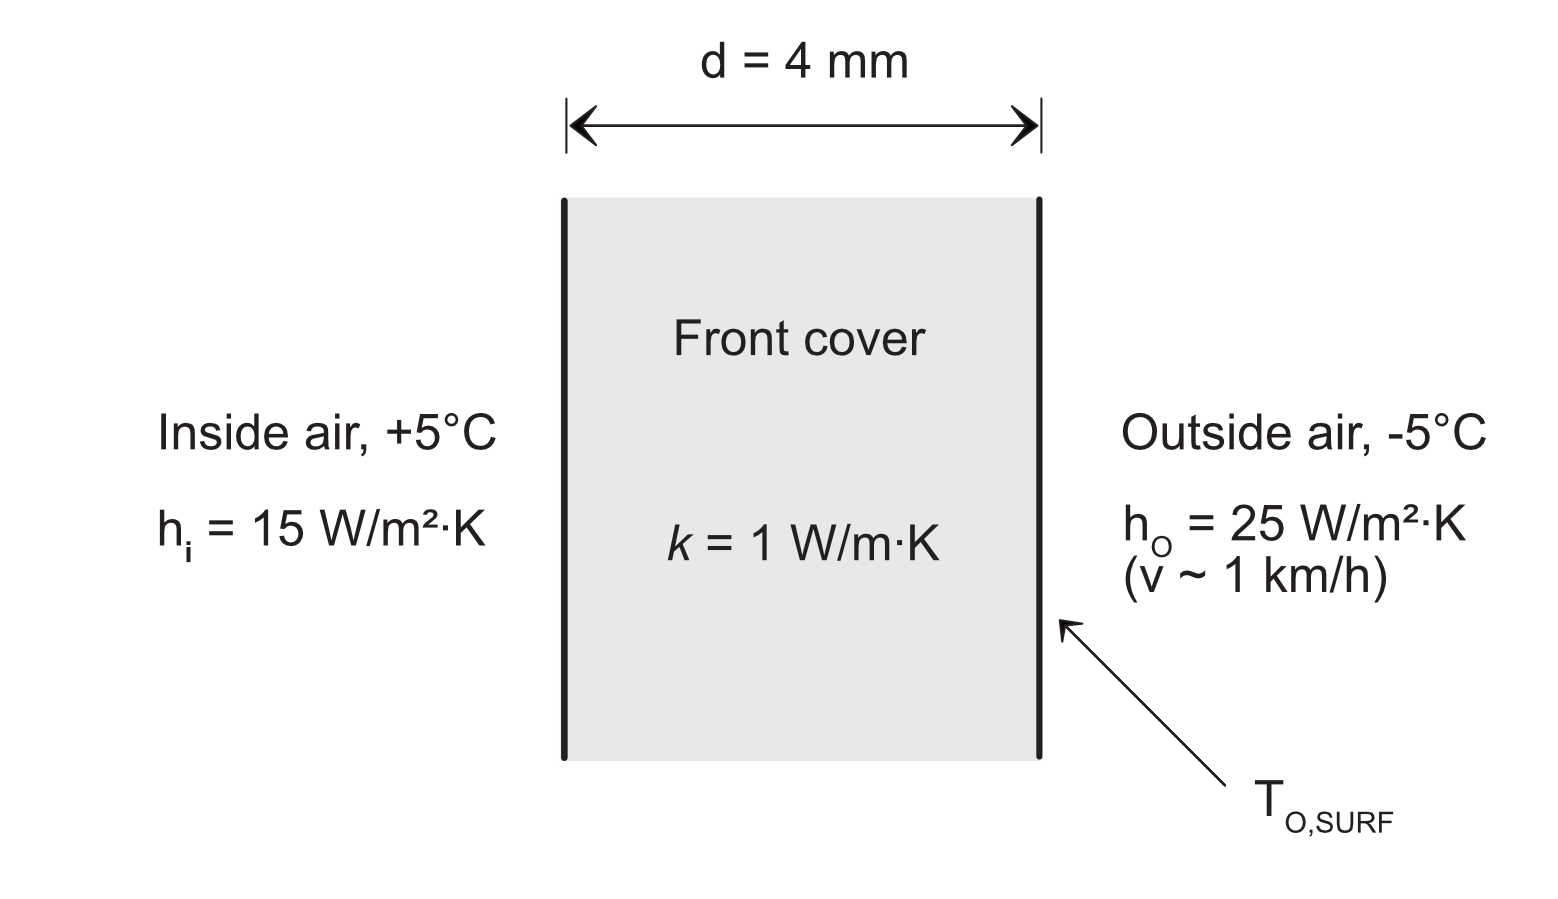
\includegraphics[scale=0.75]{\pathPics/Appendix_Windshield.png}
	\caption[PassiveHeating]{Side view sketch of a front cover}
	%\label{fig:fig1}
\end{figure}
The outer surface temperature is derived from the heat transfer rate per unit surface area, \(\dot{Q}/A\) and the thermal resistance of the front cover. The heat transfer rate per unit surface area corresponds to the power dissipated through the front cover area and can be estimated by weighting the power consumption of the sensor with the fraction of the surface area of the front cover to the surface area of the sensor. A sensor with a size of roughly 11 cm x 10 cm x 8.5 cm has a surface area of 580 \unit{cm²}. Assuming a front cover area of 45 \unit{cm^2} and an uniform dissipation loss through the sensor surface, then the sensor looses about 8 \unit{\%} of its power through the front cover:
\begin{equation}
P = 8 \% \cdot 5 \unit{W} = 0.4 \unit{W}
\end{equation}
This corresponds to a heat transfer rate per unit surface of 90 \unit{W/m²}. The temperature on the outer surface is then given by considering the heat transfer from the outer surface to the ambient air
\begin{equation}
T_{o,surf} = T_{o} + R_{o,conv}\cdot \frac{\dot{Q}}{A} = +5 \dC - 3.4 \dC = -1.4 \dC
\end{equation}
with the convection resistance \(R_{o,conv} = 1/h_{o,conv} = 0.04 \,\, \unit{m\cdot K/W}\). The temperature of the air inside the sensor can be derived in a similar manner,  
\begin{equation}
T_{i} = T_{o} + R_{tot}\cdot \frac{\dot{Q}}{A} = -5 \dC + 10 \dC = +5 \dC
\end{equation}
by considering the heat transfer through the front cover with a total resistance \(R_{tot} = 1/h_{i,conv}+d/k+1/h_{o,conv} = 0.11 \unit{m\cdot K/W}\).


\subsection{Heating Plate}


\subsection{3-D Thermal Simulation}




% bib stuff
%\bibliographystyle{unsrtnat} %%% to have citations ordered by appearance
\bibliographystyle{IEEEtran}
\bibliography{IEEEabrv, /home/hh/promo/literature/my_latest_referencer}
%\bibliography{/home/hh/promo/literature/my_latest_referencer}


%%%%%	%%% biographies
%%%%%	
%%%%%	\begin{IEEEbiography}[{\includegraphics[width=1in,height=1.25in,clip,keepaspectratio]{/home/hh/promo/conferences/hanno_pics_2020-02-17/HANNO_DSC1199_head_cutout.png}}]{Hanno Holzh{\"u}ter}
%%%%%	works as a research project manager at Ibeo Automotive Systems and is also a
%%%%%	PhD student with focus on digital signal processing in LiDAR sensors at the
%%%%%	Institute for Microelectronic Systems (IMS), Leibniz University Hanover and
%%%%%	Ibeo AS. Before joining Ibeo in 2016, Hanno worked as a scientific assistant in
%%%%%	the engineering education research group at Technical University of Hamburg
%%%%%	after finishing his master in 2015 in physics at the Georg-August-University
%%%%%	G{\"o}ttingen.
%%%%%	\end{IEEEbiography}

\end{document}








